\section{Results of Deep Kalman Filter Models}\label{sec:results}

This appendix presents the results of the vanilla DKF and of the AR DKF,
FAR DKF and BAR DKF on two kinds of data: simple sine waves, and windows
of a trajectory of the Lorenz attractor. Gaussian noise is added to the
observed part of each sequence. The model reconstructs that part and then
forecasts the following steps.

\subsection*{How to read these results}

\begin{itemize}
    \item \textbf{Errors are measured against the clean signal.} The
    reconstruction and prediction MSEs compare the model's output with
    the ground truth \emph{before} noise was added. The \enquote{MSE of
    the noise} is the error one would make by simply returning the noisy
    input.
    \item \textbf{Reconstruction at the noise level means no
    denoising.} For all the models, the reconstruction MSE is close to
    the MSE of the noise. In the figures, the
    reconstruction follows the noisy input point by point rather than the
    clean curve. The inference network passes each observation, noise
    included, through the latent state, and the decoder reproduces it.
    A good reconstruction MSE is therefore \emph{not} evidence that the
    model has learned the dynamics; the forecasting error is the
    informative quantity.
    \item \textbf{Forecasts are single sampled paths.} \code{predict}
    samples one latent trajectory and one path of the dynamics. Its error
    includes sampling noise and would be lower for the mean of the
    predictive distribution.
    \item \textbf{Repeated runs.} Each Lorenz experiment was trained
    four times. The figures of each dataset show the first run; the
    summary at the end of this appendix gives the mean and the spread
    over the four runs. The sine-wave experiments were trained once.
\end{itemize}

\subsection*{DKF with Simple Sine Waves}

The vanilla DKF was tested on two sine-wave datasets with different
frequencies. It follows the observed part of the sequences closely, but
its forecasts lose track of the signal. With $f=1$ they flatten out and
lose the amplitude; with $f=2$ they keep oscillating at roughly the right
frequency but drift out of phase within one or two periods. The
transition model alone has not learned the periodic dynamics.

\begin{figure}[ht!]
    \centering
    \begin{subfigure}[b]{0.49\textwidth}
        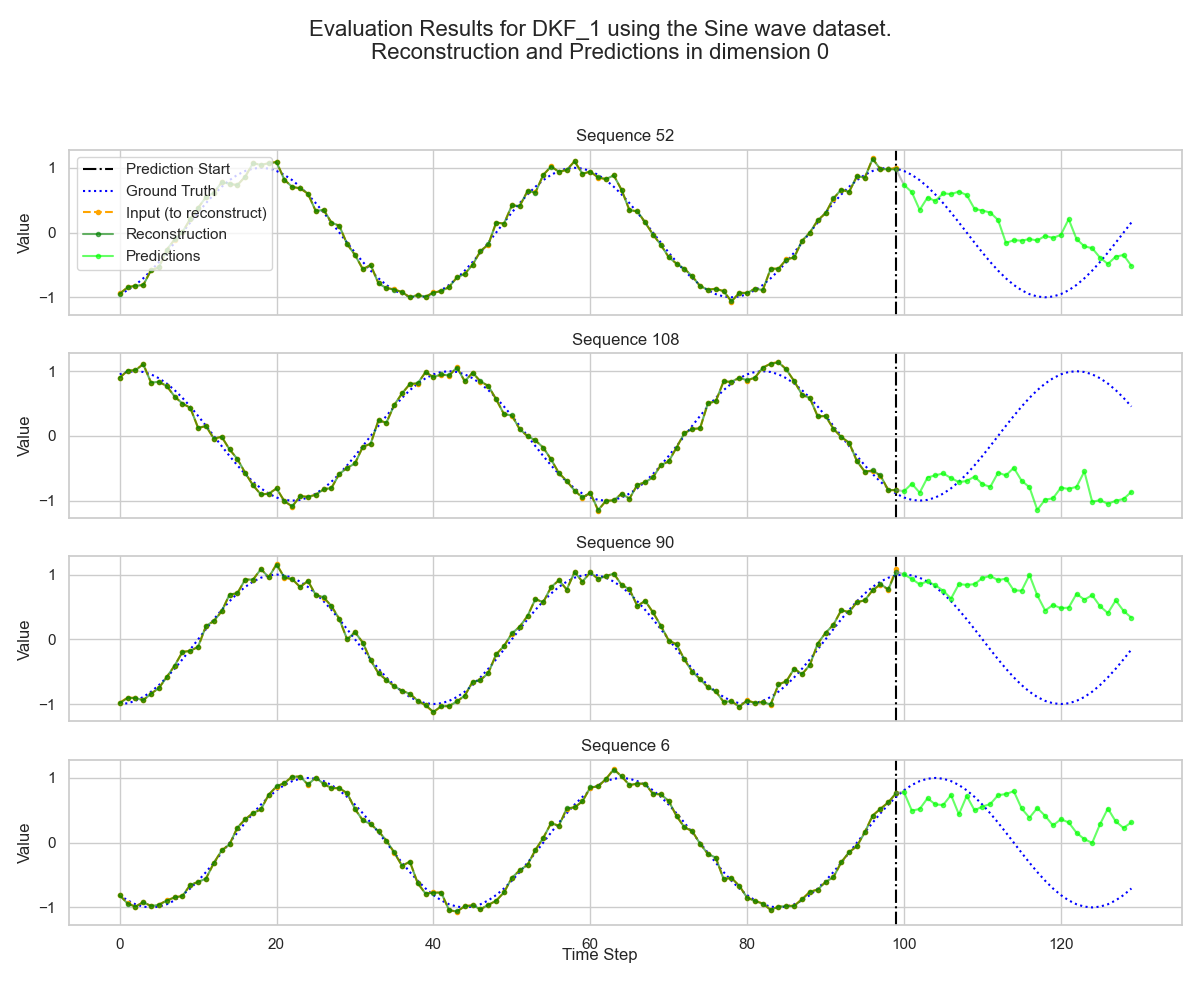
\includegraphics[width=\textwidth]{./Images/DKF_sine_wave_1.png}
        \caption{DKF on sine wave with $f=1$.}
        \label{fig:dkf_sine_wave_1}
    \end{subfigure}
    \hfill
    \begin{subfigure}[b]{0.49\textwidth}
        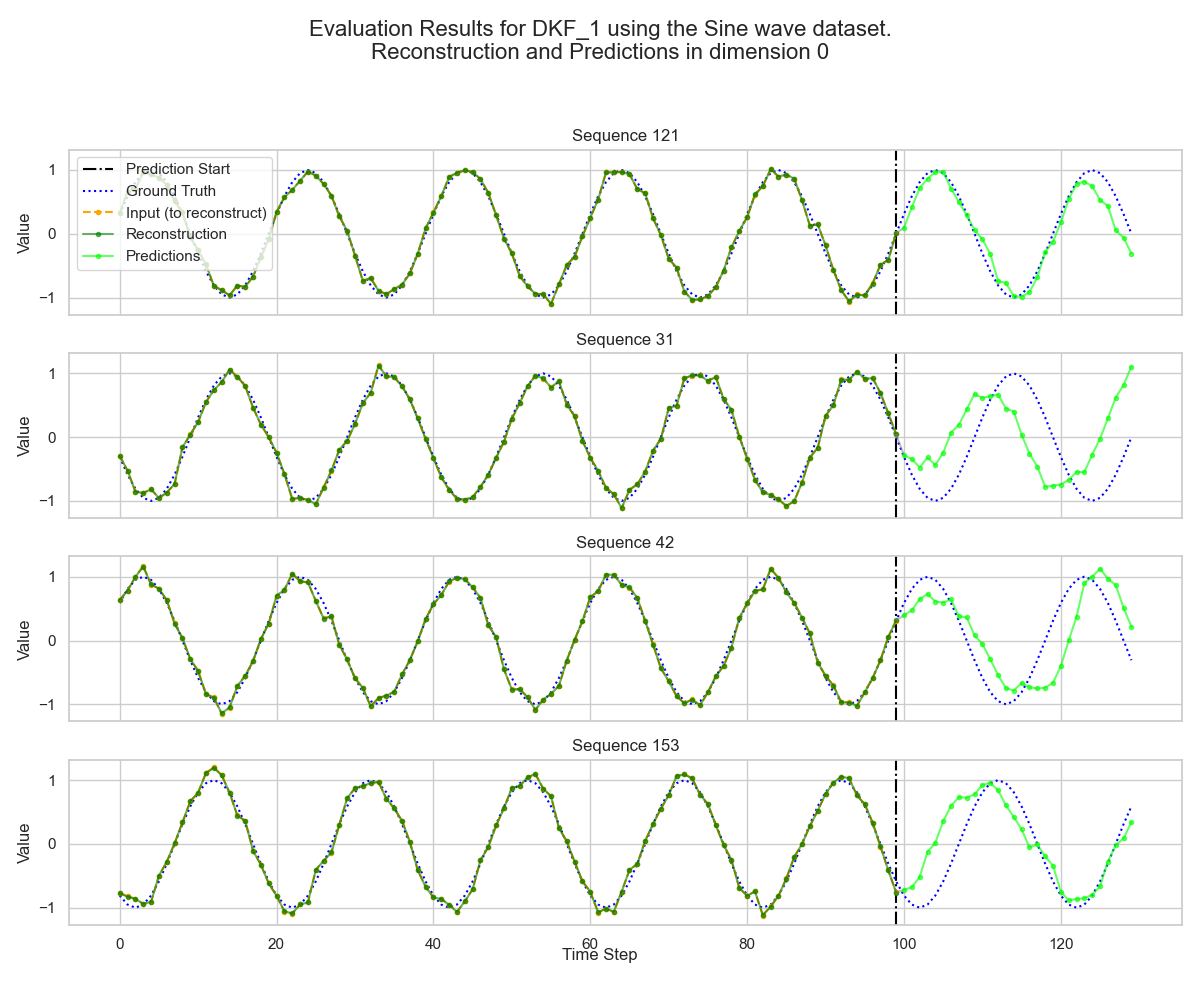
\includegraphics[width=\textwidth]{./Images/DKF_sine_wave_2.png}
        \caption{DKF on sine wave with $f=2$.}
        \label{fig:dkf_sine_wave_2}
    \end{subfigure}
    \caption{DKF reconstruction and prediction on two sine-wave
    datasets.}
    \label{fig:dkf_sine_wave_results}
\end{figure}

\subsection*{AR DKF with Simple Sine Waves}
    
    The AR DKF was tested on the same sine wave datasets as
    for the DKF.
    The AR DKF forecasts both sine waves far better than the vanilla DKF:
    the forecasts keep the phase, the frequency and the amplitude of the
    signal over the whole prediction window. The prediction MSE is
    $0.876$ for the DKF and $0.0052$ for the AR DKF with $f=1$, and
    $0.571$ and $0.0094$ with $f=2$ (Figure~\ref{fig:sine_mse_comparison}).
    For a sine wave of amplitude 1, always predicting $0$ would give an MSE
    of $0.5$: on both datasets the DKF forecasts are worse than this
    trivial predictor, while the AR DKF forecasts have an error of the
    same order as the noise of the observations.
    The difference is large enough to be conclusive even with a single
    run. It supports the idea behind the AR DKF: giving the transition
    model direct access to the history lets it carry the information
    needed for forecasting.
    
    \begin{figure}[ht!]
        \centering
        \begin{subfigure}[b]{0.49\textwidth}
            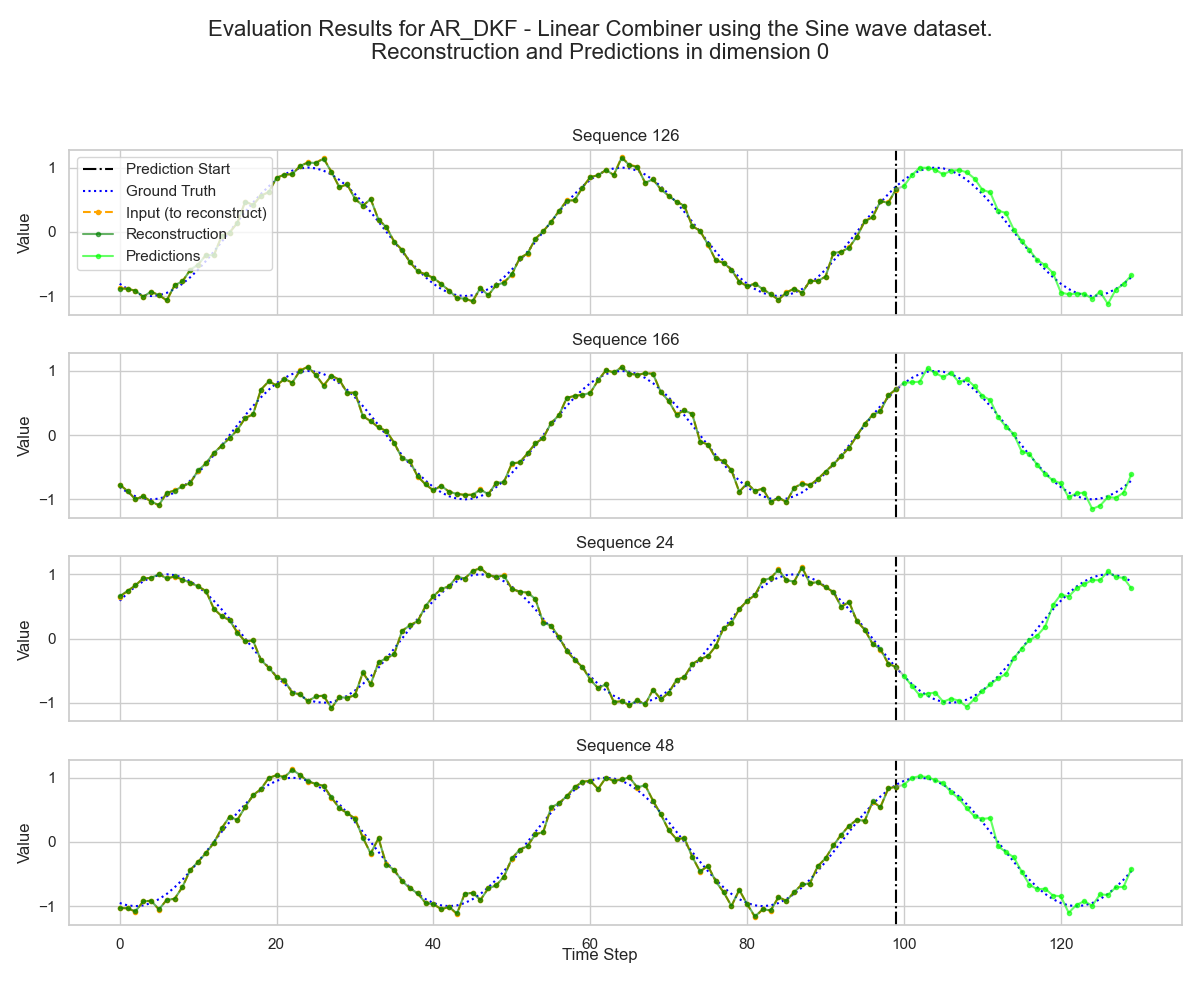
\includegraphics[width=\textwidth]{./Images/AR_DKF_sine_wave_1.png}
            \caption{AR DKF on sine wave with $f=1$.}
            \label{fig:ar_dkf_sine_wave_1}
        \end{subfigure}
        \hfill
        \begin{subfigure}[b]{0.49\textwidth}
            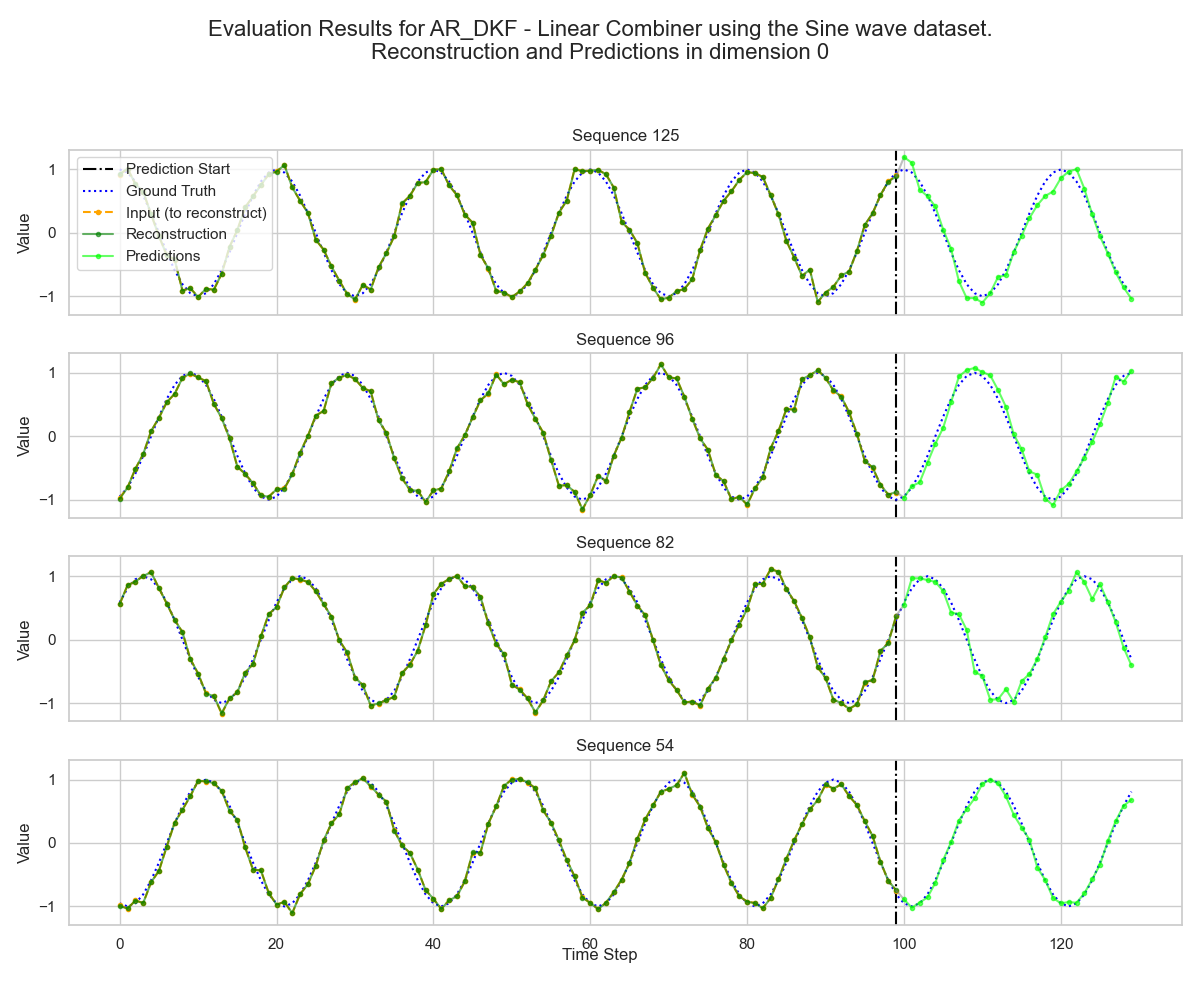
\includegraphics[width=\textwidth]{./Images/AR_DKF_sine_wave_2.png}
            \caption{AR DKF on sine wave with $f=2$.}
            \label{fig:ar_dkf_sine_wave_2}
        \end{subfigure}
        \caption{Examples of AR DKF Reconstruction and Prediction
        on two simple sine wave datasets.}
        \label{fig:ar_dkf_sine_wave_results}
    \end{figure}

    \begin{figure}[ht!]
        \centering
        \begin{subfigure}[b]{0.49\textwidth}
            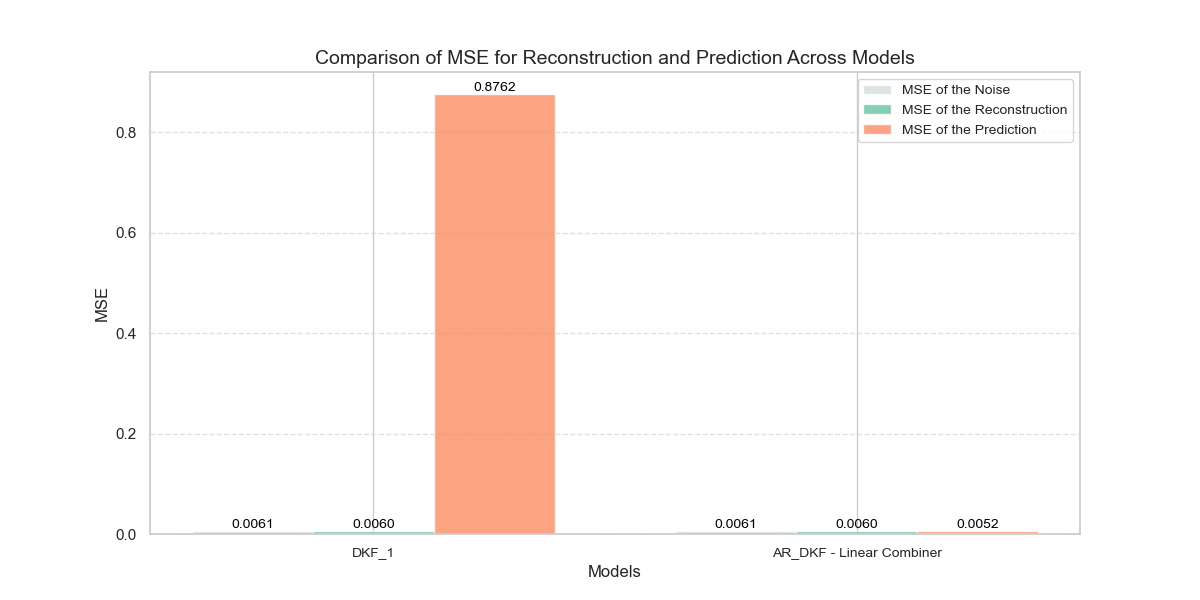
\includegraphics[width=\textwidth]{./Images/sine_mse_comparison_1.png}
            \caption{Sine wave with $f=1$.}
        \end{subfigure}
        \hfill
        \begin{subfigure}[b]{0.49\textwidth}
            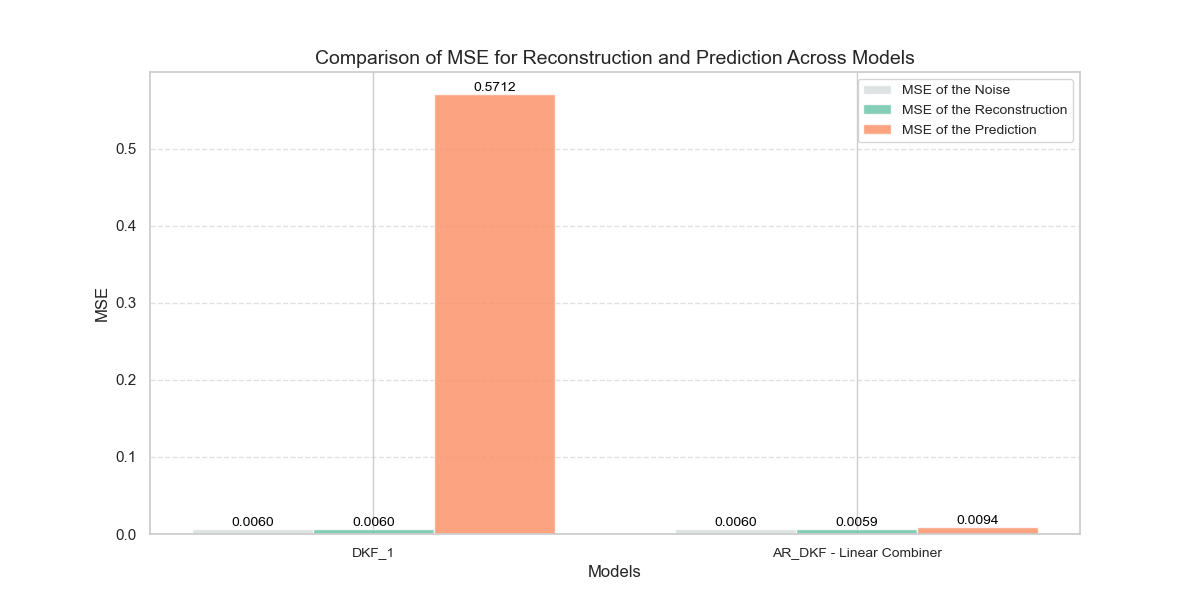
\includegraphics[width=\textwidth]{./Images/sine_mse_comparison_2.png}
            \caption{Sine wave with $f=2$.}
        \end{subfigure}
        \caption{Reconstruction and prediction MSE of the DKF and the
        AR DKF on the two sine-wave datasets.}
        \label{fig:sine_mse_comparison}
    \end{figure}
    
    \subsection*{Comparison of AR DKF, FAR DKF, and
    BAR DKF on Lorenz Attractor}
    
    The AR DKF, FAR DKF, and BAR DKF
    were compared using three sets of data from the Lorenz attractor.
    The datasets were designed to test the models' ability to
    generalize under varying degrees of dissimilarity between training
    and testing data. Each experiment was repeated four times with the
    same settings; the figures below show the first run.
    
    \subsubsection*{Configurations}
    All the subsequent results are obtained with configurations
    given in the tables below.\\
    
    %- - - - - - - - - - - - - - - - - - - - - - - - - - - - 
    \begin{minipage}{0.48\textwidth}
        \centering
        \small
        \label{tab:args_config}
        \captionof{table}{Args Configuration}
        \begin{tabular}{|l|l|}
        \hline
        \textbf{Parameter} & \textbf{Value} \\ \hline
        dataset & lorenz \\ \hline
        lorenz\_initial\_point & 2, 1, 1 \\ \hline
        lorenz\_points & 20000 \\ \hline
        lorenz\_range & Dataset 1: [4500, 6500] \\
        & Dataset 2: [8600, 10500]\\
        & Dataset 3: [11000, 13000]\\ \hline
        loss\_function & weighted\_mse \\ \hline
        noise\_var & 0.006 \\ \hline
        normalization\_type & standardize \\ \hline
        train\_seq\_len & 100 \\ \hline
        test\_seq\_len (prediction) & 100 \\ \hline
        \end{tabular}
     %\end{table}
    \end{minipage}
    \hfill
    \begin{minipage}{0.45\textwidth}
        \centering
            \label{tab:training_config_config}
            \captionof{table}{Training Configuration}
            \begin{tabular}{|l|l|}
            \hline
            \textbf{Parameter} & \textbf{Value} \\ \hline
            learning\_rate & 0.001 \\ \hline
            num\_epochs & 120 \\ \hline
            pred\_batch\_size & 32 \\ \hline
            train\_batch\_size & 32 \\ \hline
            val\_batch\_size & 16 \\ \hline
            \end{tabular}
        %\end{table} 
    \end{minipage}
    
    \begin{table}[h!]
    \centering
    \caption{Models Configuration}
    \label{tab:models_config_config}
    \begin{tabular}{|l|l|l|l|}
    \hline
    \diagbox[width=\dimexpr \textwidth/4 + 4\tabcolsep\relax,height=0.7cm]
    {\textbf{Parameter}}{\textbf{Model}}
    & \textbf{AR DKF} & \textbf{FAR DKF} & 
    \textbf{BAR DKF} \\ \hline
    activation & tanh & tanh & tanh \\ \hline
    combiner\_alpha & 0.5 & 0.5, 0.5 & 0.5 \\ \hline
    combiner\_alpha\_init & 0.1 & 0.1, 0.1 & 0.1 \\ \hline
    combiner\_layers\_dim & 64 & 64 & 64 \\ \hline
    combiner\_learnable\_alpha & Yes & Yes, Yes & Yes \\ \hline
    combiner\_output\_dim & 64 & 64 & 64 \\ \hline
    combiner\_type & linear & linear & linear \\ \hline
    decoder\_layers\_dim & 64, 32 & 64, 32 & 64, 32 \\ \hline
    device & cpu & cpu & cpu \\ \hline
    dropout\_p & 0.0 & 0.0 & 0.0 \\ \hline
    encoder\_layers\_dim & 64 & 64 & 64 \\ \hline
    latent\_transition\_layers\_dim & 64 & 64 & 64 \\ \hline
    learnable\_init\_x & No & No & No \\ \hline
    learnable\_init\_z & Yes & Yes & Yes \\ \hline
    pz\_f\_rnn\_hidden\_size & 64 & 64 & 64 \\ \hline
    pz\_f\_rnn\_num\_layers & 1 & 1 & 1 \\ \hline
    q\_b\_rnn\_hidden\_size & 64 & 64 & 64 \\ \hline
    q\_b\_rnn\_num\_layers & 1 & 1 & 1 \\ \hline
    x\_dim & 3 & 3 & 3 \\ \hline
    z\_dim & 16 & 16 & 16 \\ \hline
    q\_f\_rnn\_hidden\_size &  & 64 &  \\ \hline
    q\_f\_rnn\_num\_layers &  & 1 &  \\ \hline
    
    \end{tabular}
    \end{table}
    
    %- - - - - - - - - - - - - - - - - - - - - - - - - - - - 
    
    \subsubsection*{Dataset 1}
    
    The dataset (\textit{before the addition of Gaussian noise}) is shown
    in the figure \ref{fig:dataset_1_partial_data} below.\\
    
    \begin{figure}[ht!]
        \centering
        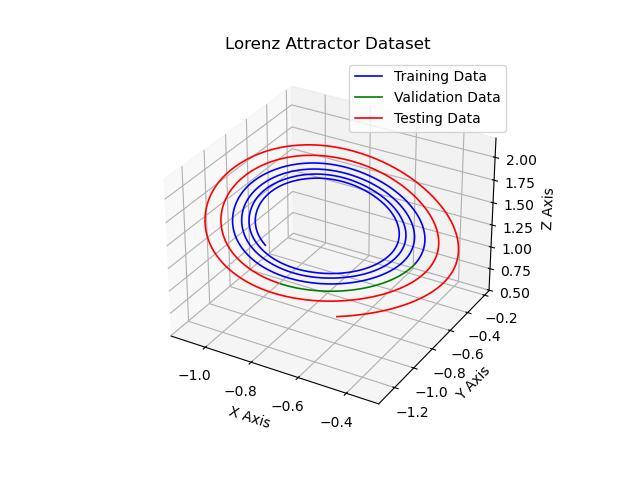
\includegraphics[width=0.75\textwidth]
        {./Images/Dataset_1/partial_data.png}
        \caption{Lorenz attractor - Range [4500, 6500] }
        \label{fig:dataset_1_partial_data}
    \end{figure}
    %
    \FloatBarrier
    
    Figure \ref{fig:dataset_1_AR_DKF_1_all_dims} below shows the results
    of the AR DKF model for four sequences from the dataset in
    each dimension.
    
    \begin{figure}[ht!]
        \centering
        \begin{minipage}{0.31\textwidth}
            \centering
            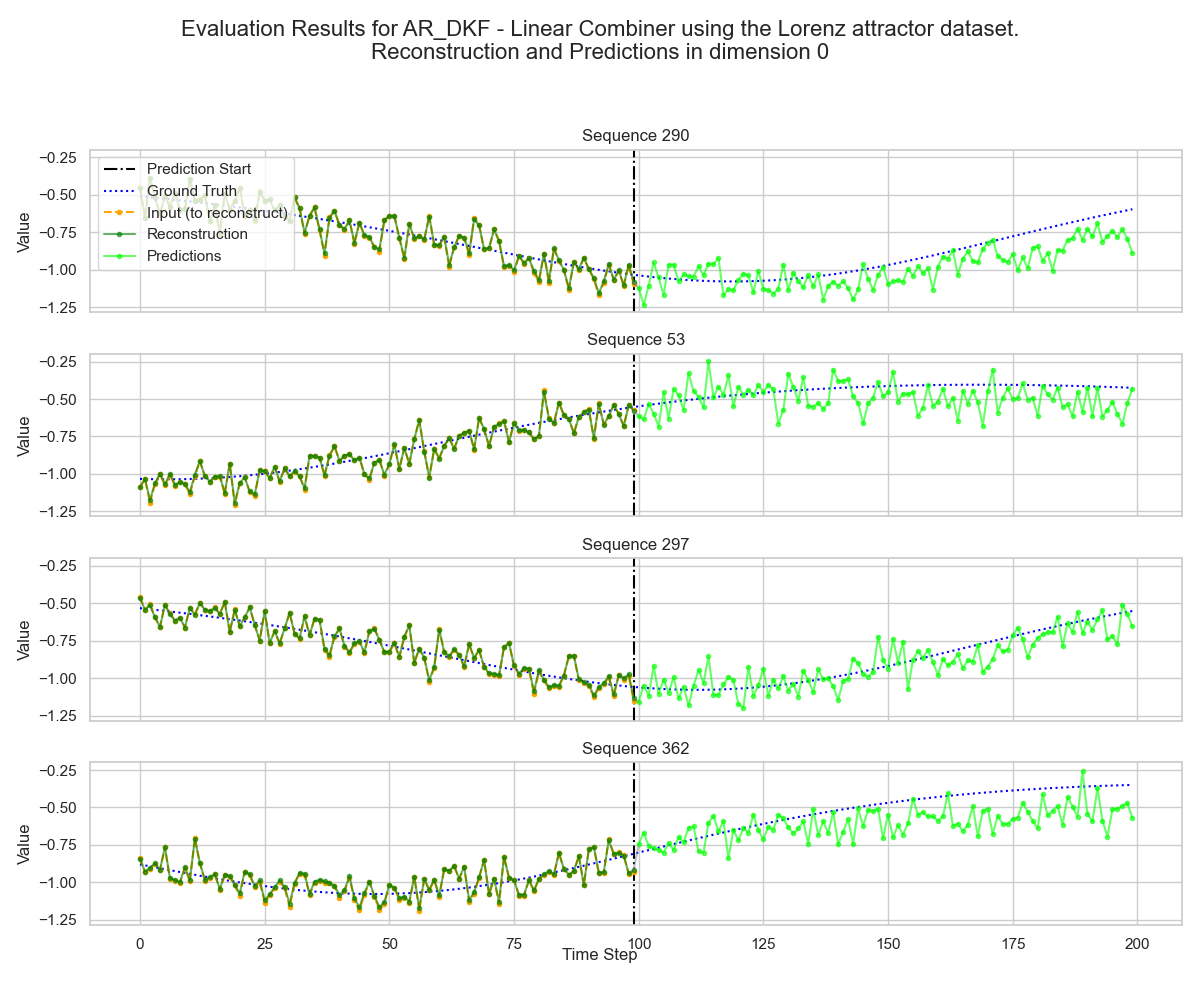
\includegraphics[width=1\textwidth]{./Images/Dataset_1/AR_DKF_1_dim_0.png}
            \subcaption{Reconstruction and Prediction in the 1st dimension.}
            \label{fig:dataset_1_AR_DKF_1_dim_0}
        \end{minipage}
        \hfill
        \begin{minipage}{0.31\textwidth}
            \centering
            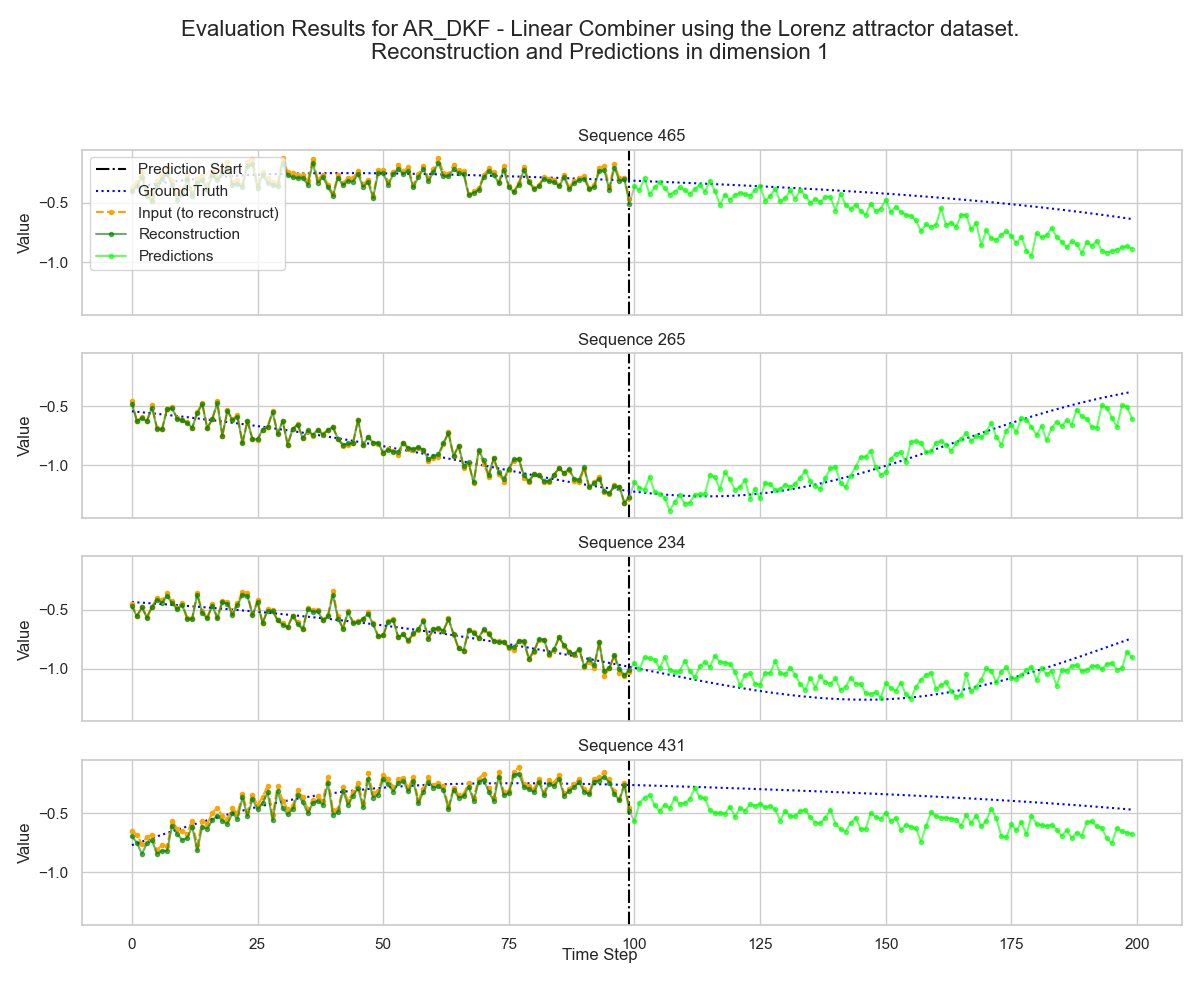
\includegraphics[width=1\textwidth]{./Images/Dataset_1/AR_DKF_1_dim_1.png}
            \subcaption{Reconstruction and Prediction in the 2nd dimension.}
            \label{fig:dataset_1_AR_DKF_1_dim_1}
        \end{minipage}
        \hfill
        \begin{minipage}{0.31\textwidth}
            \centering
            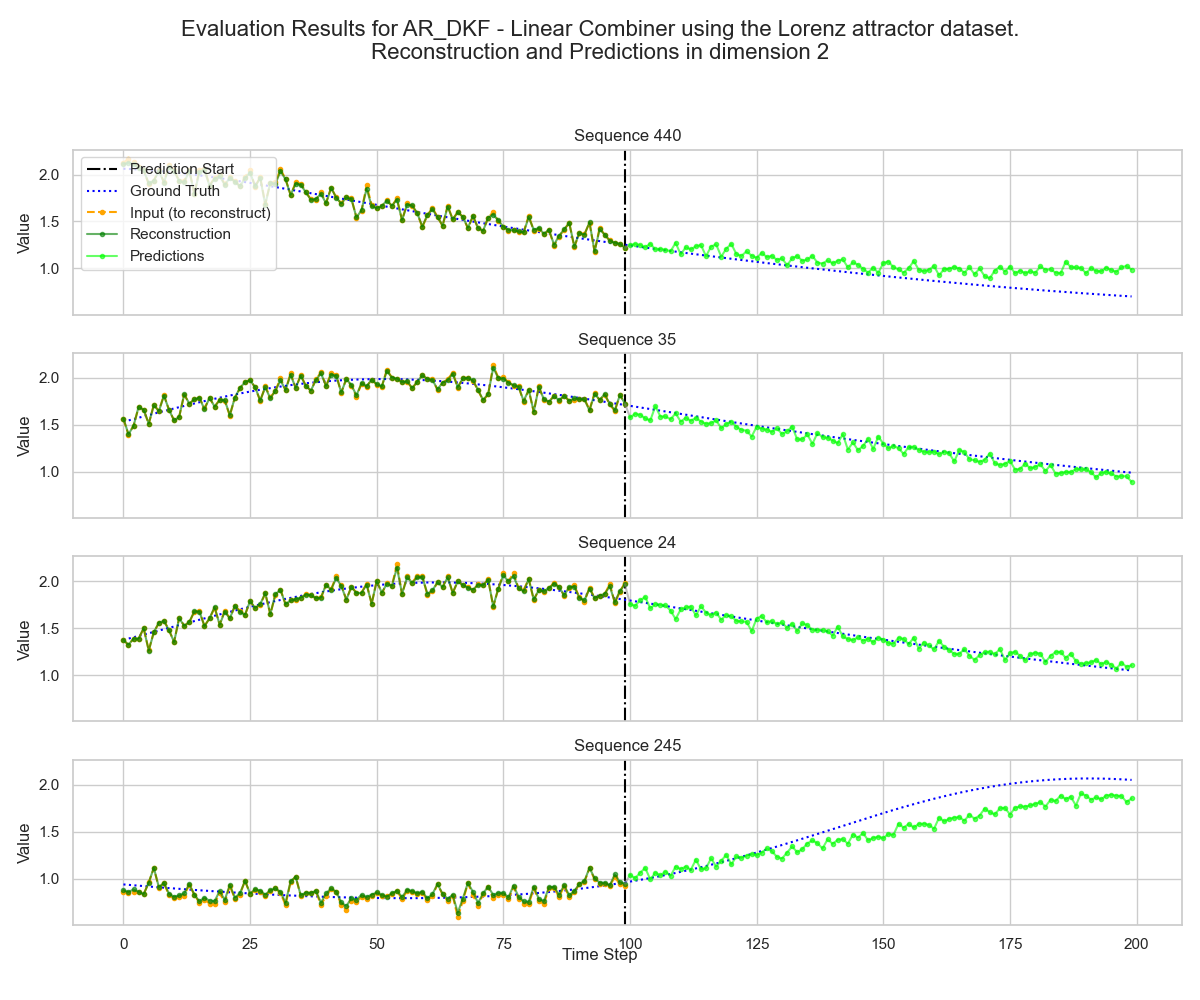
\includegraphics[width=1\textwidth]{./Images/Dataset_1/AR_DKF_1_dim_2.png}
            \subcaption{Reconstruction and Prediction in the 3rd dimension.}
            \label{fig:dataset_1_AR_DKF_1_dim_2}
        \end{minipage}
        \caption{Examples of Reconstruction and Prediction for the
        AR DKF model.}
        \label{fig:dataset_1_AR_DKF_1_all_dims}
    \end{figure}
    
    Figure \ref{fig:dataset_1_FAR_DKF_1_all_dims} below shows the results
    of the FAR DKF model on the same sequences.
    
    \begin{figure}[ht!]
        \centering
        \begin{minipage}{0.31\textwidth}
            \centering
            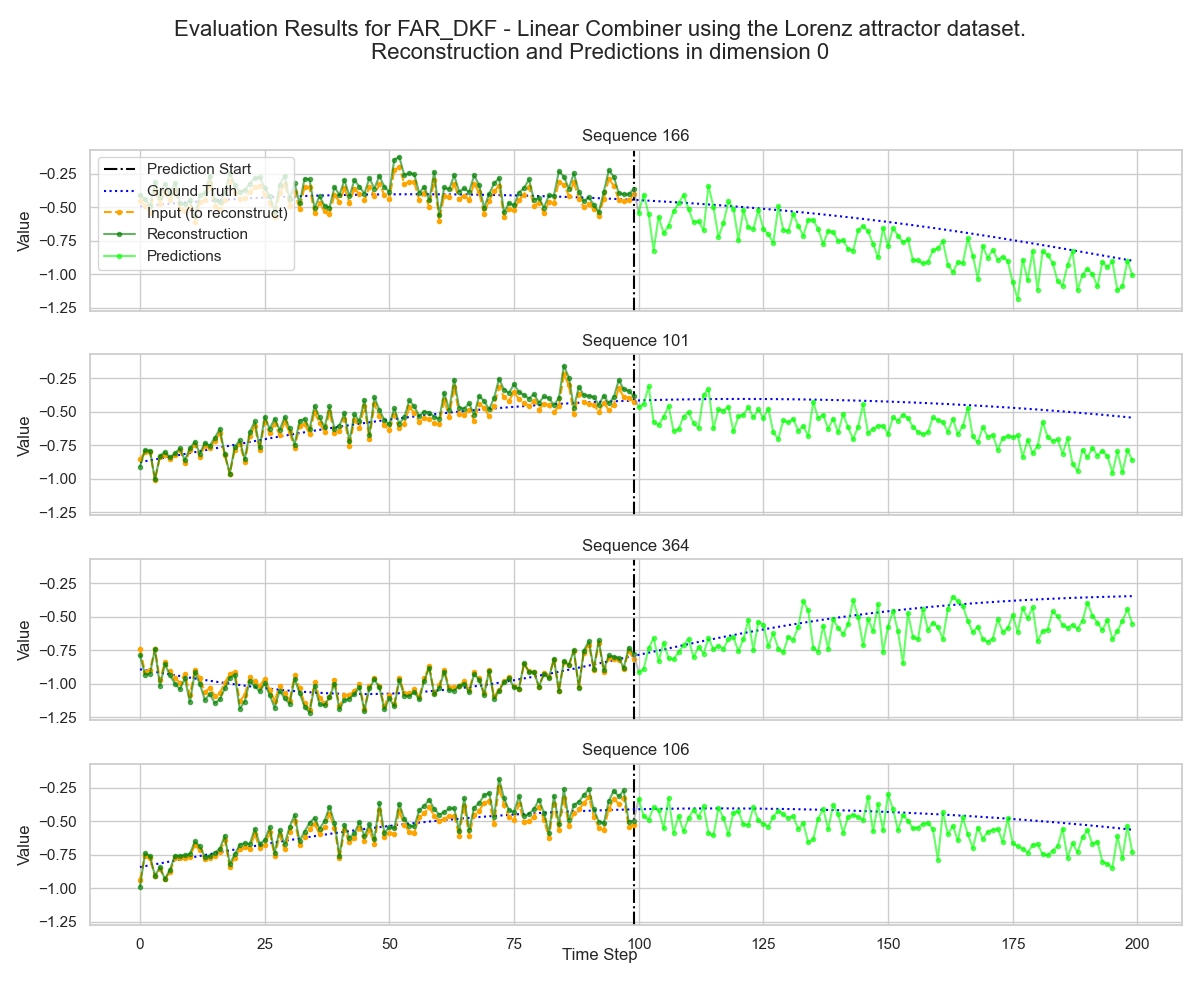
\includegraphics[width=1\textwidth]{./Images/Dataset_1/FAR_DKF_1_dim_0.png}
            \subcaption{Reconstruction and Prediction in the 1st dimension.}
            \label{fig:dataset_1_FAR_DKF_1_dim_0}
        \end{minipage}
        \hfill
        \begin{minipage}{0.31\textwidth}
            \centering
            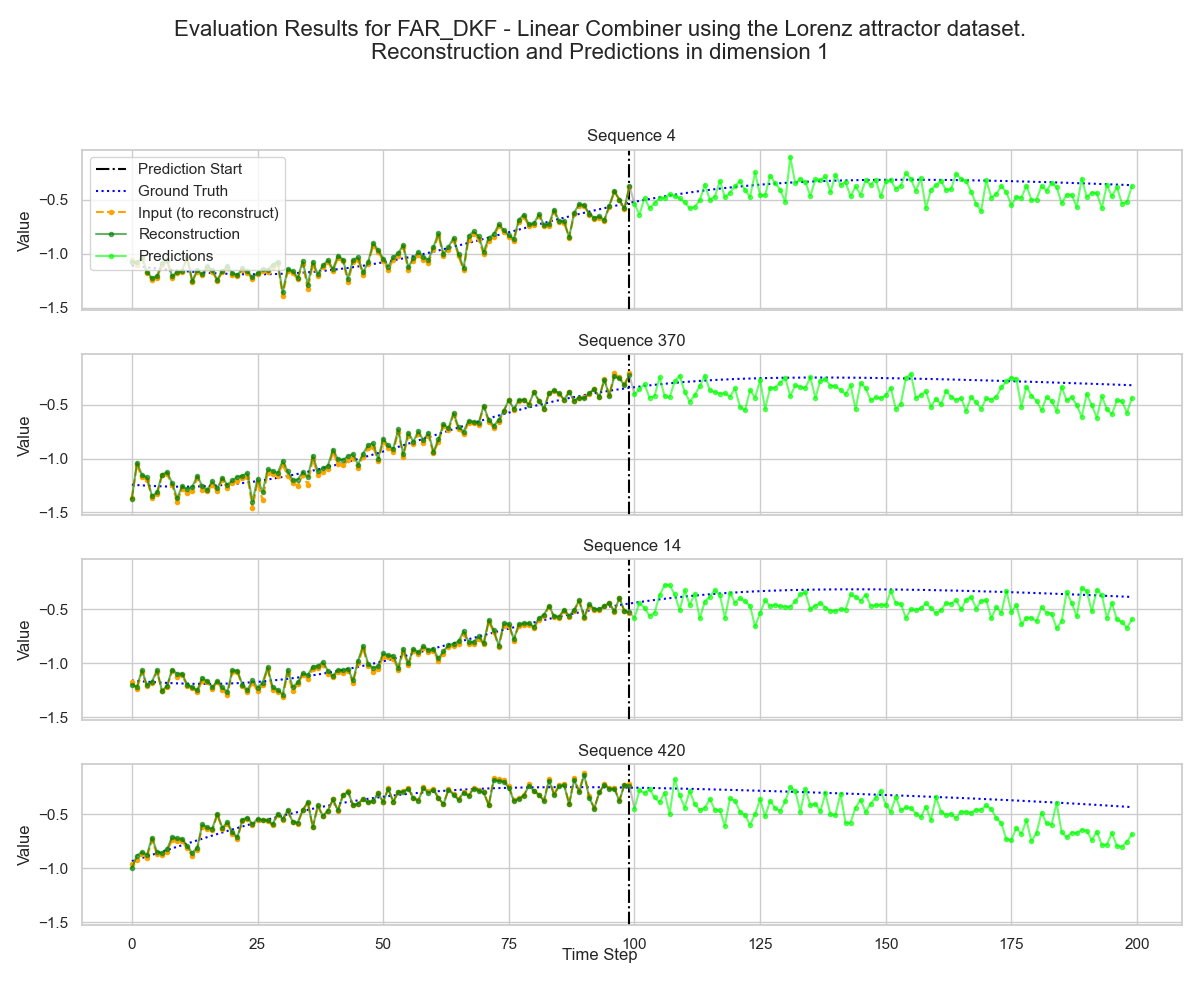
\includegraphics[width=1\textwidth]{./Images/Dataset_1/FAR_DKF_1_dim_1.png}
            \subcaption{Reconstruction and Prediction in the 2nd dimension.}
            \label{fig:dataset_1_FAR_DKF_1_dim_1}
        \end{minipage}
        \hfill
        \begin{minipage}{0.31\textwidth}
            \centering
            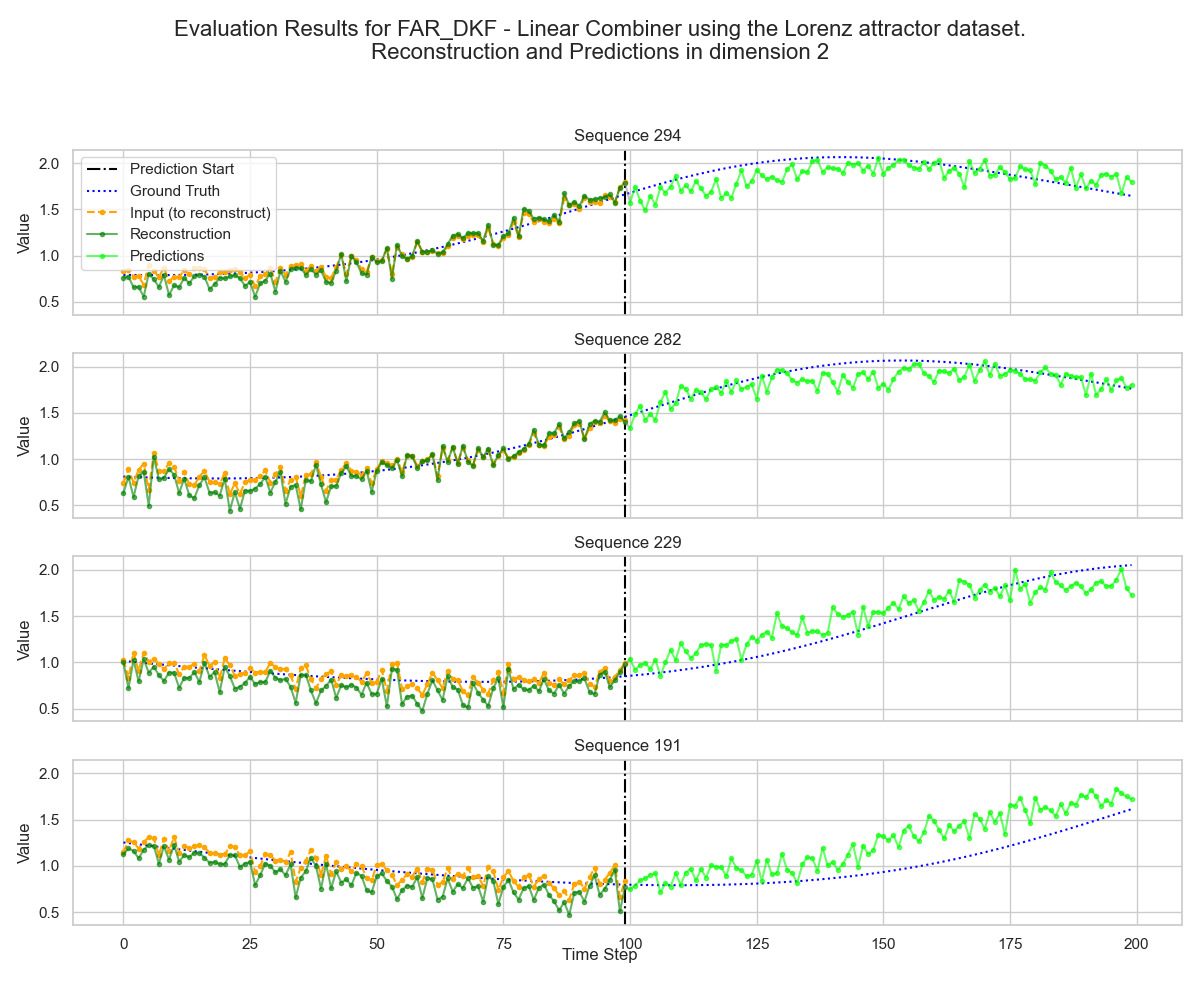
\includegraphics[width=1\textwidth]{./Images/Dataset_1/FAR_DKF_1_dim_2.png}
            \subcaption{Reconstruction and Prediction in the 3rd dimension.}
            \label{fig:dataset_1_FAR_DKF_1_dim_2}
        \end{minipage}
        \caption{Examples of Reconstruction and Prediction for the
        FAR DKF model.}
        \label{fig:dataset_1_FAR_DKF_1_all_dims}
    \end{figure}
    
    And Figure \ref{fig:dataset_1_BAR_DKF_1_all_dims} shows the results
    of the BAR DKF.
    
    \begin{figure}[ht!]
        \centering
        \begin{minipage}{0.31\textwidth}
            \centering
            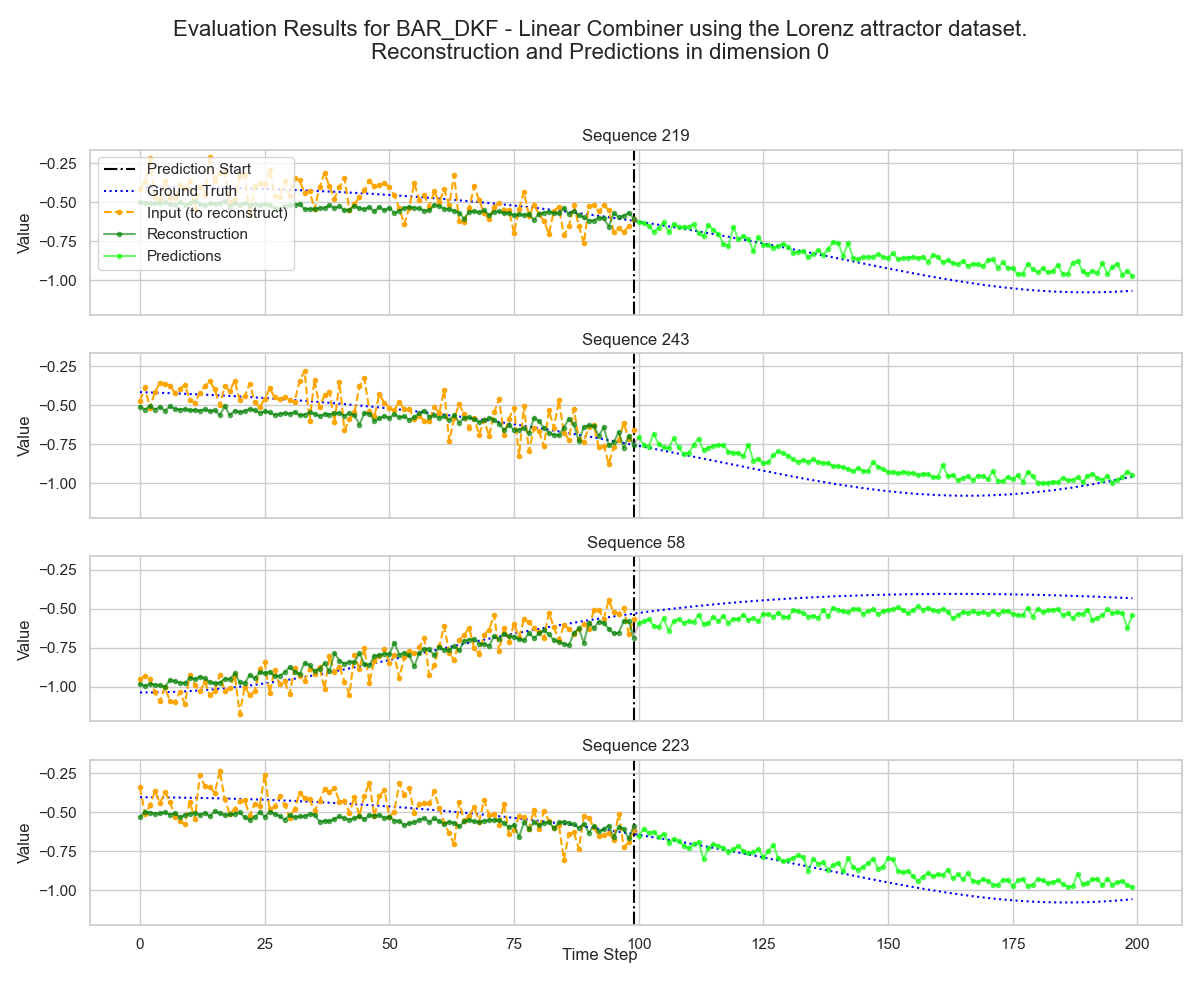
\includegraphics[width=1\textwidth]{./Images/Dataset_1/BAR_DKF_1_dim_0.png}
            \subcaption{Reconstruction and Prediction in the 1st dimension.}
            \label{fig:dataset_1_BAR_DKF_1_dim_0}
        \end{minipage}
        \hfill
        \begin{minipage}{0.31\textwidth}
            \centering
            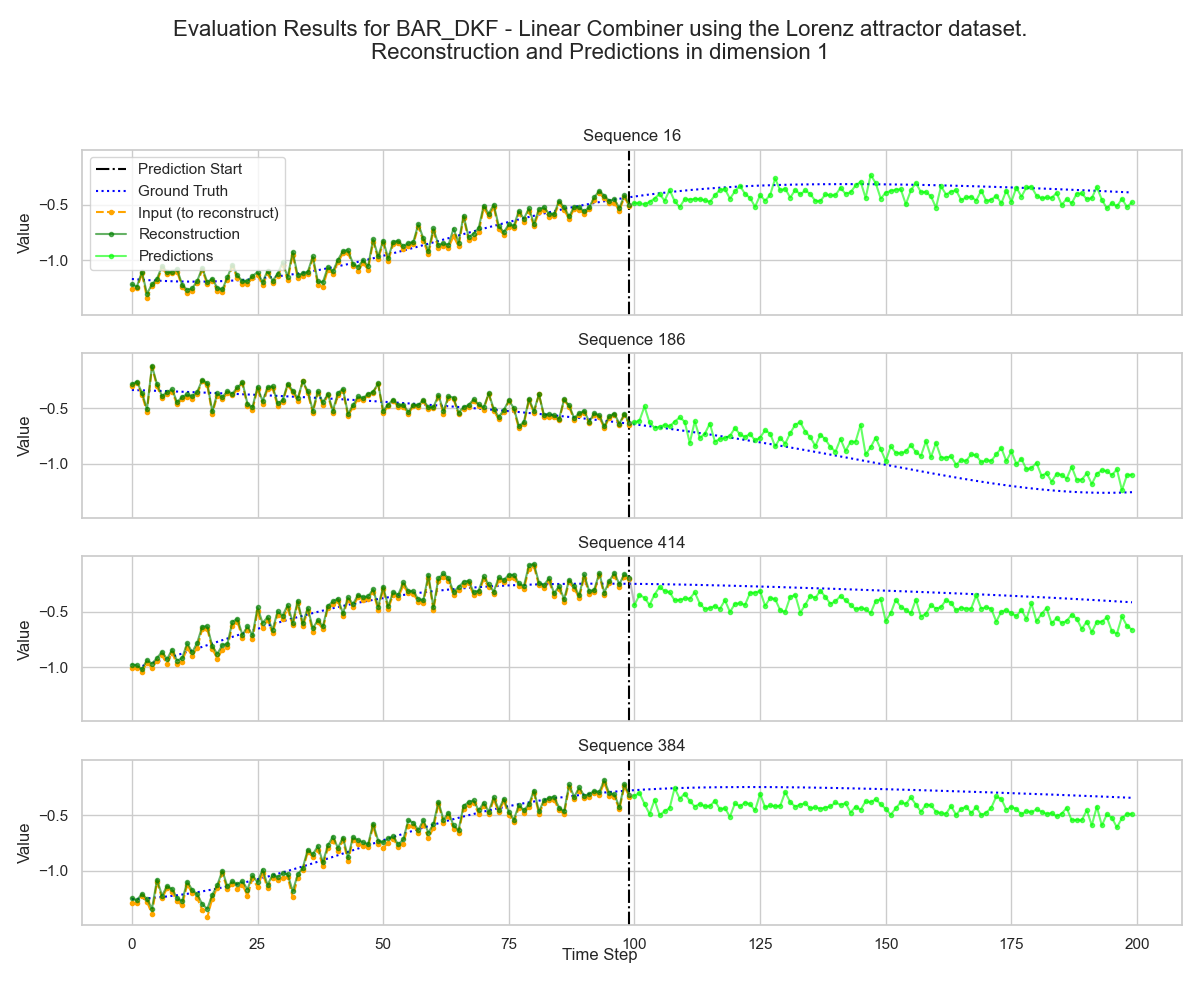
\includegraphics[width=1\textwidth]{./Images/Dataset_1/BAR_DKF_1_dim_1.png}
            \subcaption{Reconstruction and Prediction in the 2nd dimension.}
            \label{fig:dataset_1_BAR_DKF_1_dim_1}
        \end{minipage}
        \hfill
        \begin{minipage}{0.31\textwidth}
            \centering
            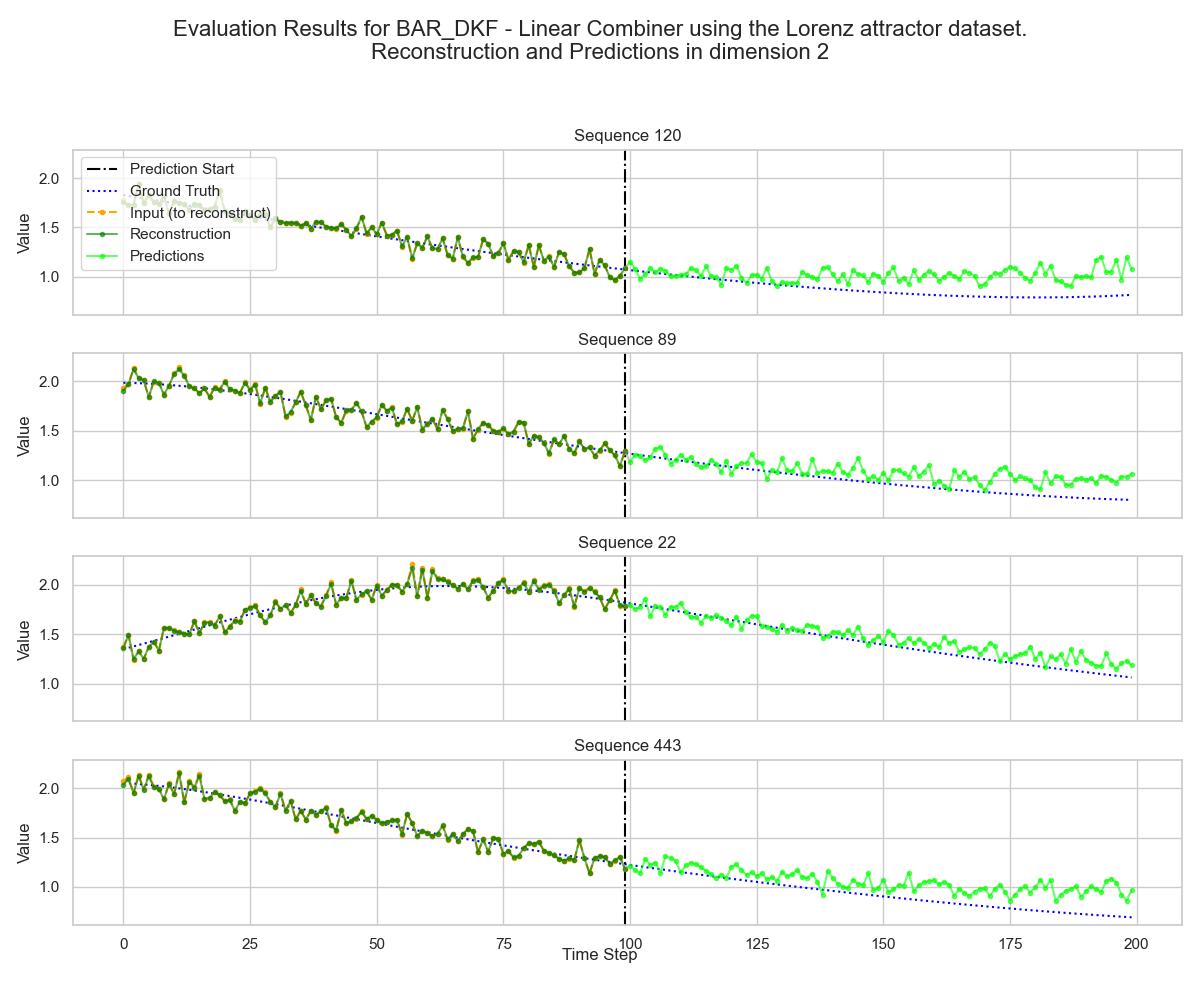
\includegraphics[width=1\textwidth]{./Images/Dataset_1/BAR_DKF_1_dim_2.png}
            \subcaption{Reconstruction and Prediction in the 3rd dimension.}
            \label{fig:dataset_1_BAR_DKF_1_dim_2}
        \end{minipage}
        \caption{Examples of Reconstruction and Prediction for the
        BAR DKF model.}
        \label{fig:dataset_1_BAR_DKF_1_all_dims}
    \end{figure}
    
    \FloatBarrier
    
    Figure \ref{fig:dataset_1_mse_comparison} below shows a
    comparison of the Mean Square Error for the reconstruction
    and the prediction tasks for each model. The MSE of the noise
    is plotted for reference.\\
    The three models have prediction errors of the same order: 0.0269
    for the AR DKF, 0.0309 for the FAR DKF and 0.0218 for the BAR DKF.
    The AR DKF and the BAR DKF reconstruct at the noise level. The FAR DKF
    reconstruction error (0.0092) is above it, i.e.\ worse than simply
    returning the noisy input.
    
    \begin{figure}[ht!]
        \centering
        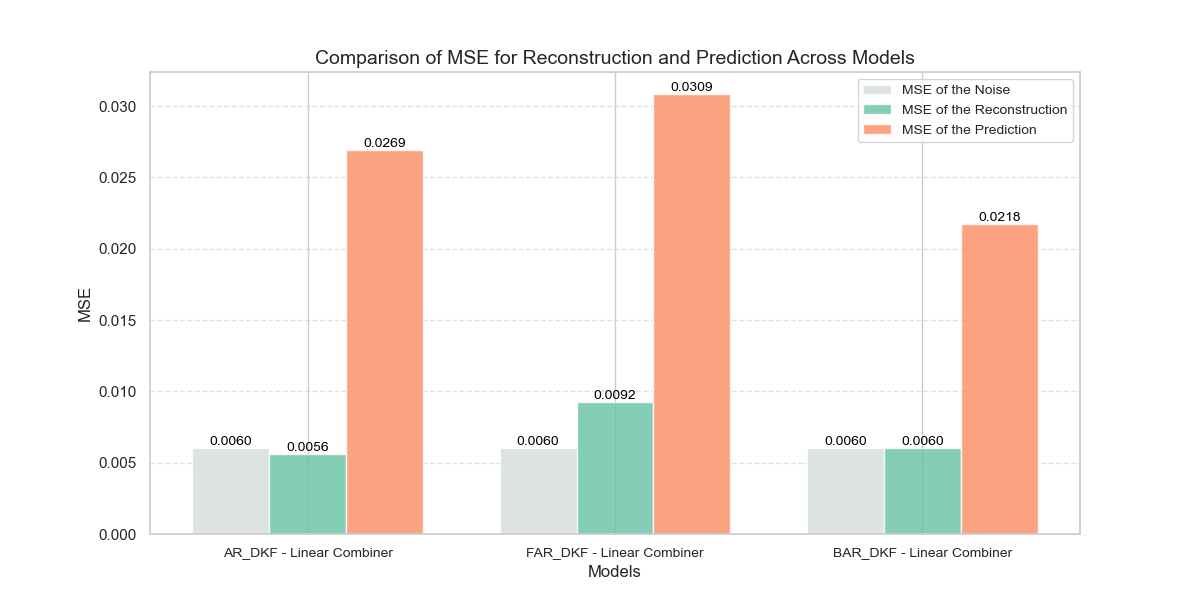
\includegraphics[width=0.75\textwidth]
        {./Images/Dataset_1/mse_comparison.png}
        \caption{Reconstruction and Prediction MSE Comparison for
        AR DKF, FAR DKF, and BAR DKF
        on dataset 1.}
        \label{fig:dataset_1_mse_comparison}
    \end{figure}
    
    Figure \ref{fig:dataset_1_mse_pred_comparison} below shows a
    comparison of the Mean Square Error for each predicted point
    for each model.\\
    As expected, the error grows with the forecasting horizon, since
    errors accumulate along the sampled path.
    
    \begin{figure}[ht!]
        \centering
        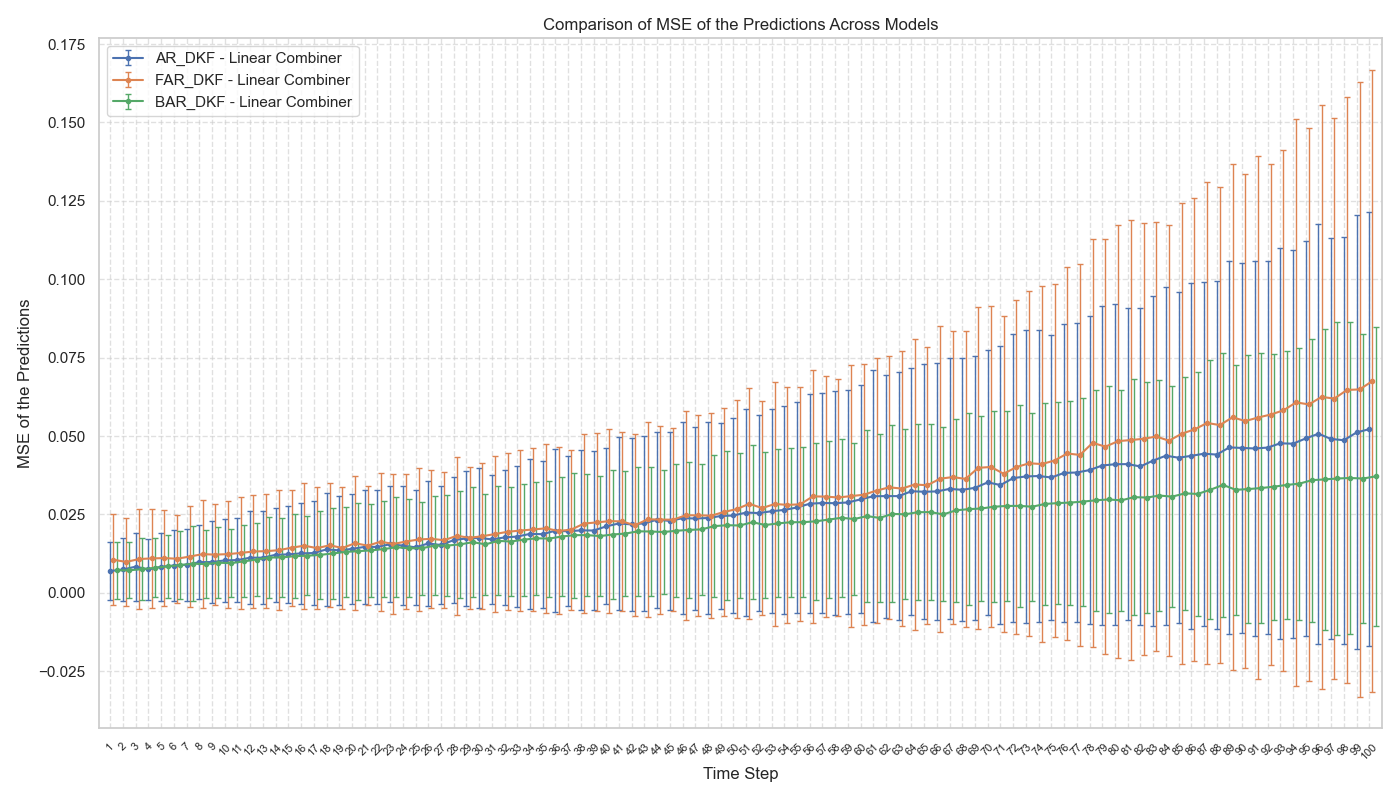
\includegraphics[width=1\textwidth]
        {./Images/Dataset_1/mse_pred_comparison.png}
        \caption{MSE Comparison for AR DKF, FAR DKF, and
        BAR DKF for each prediction points of test sequences of
        dataset 1.}
        \label{fig:dataset_1_mse_pred_comparison}
    \end{figure}
    %
    \FloatBarrier
    The same comparisons were done on the dataset 2 and 3.
    The results are shown below.
    %- - - - - - - - - - - - - - - - - - - - - - - - - - - - 
    \subsubsection*{Dataset 2}
    
    The dataset (\textit{before the addition of Gaussian noise}) is shown
    in figure \ref{fig:dataset_2_partial_data}.
    
    \begin{figure}[ht!]
        \centering
        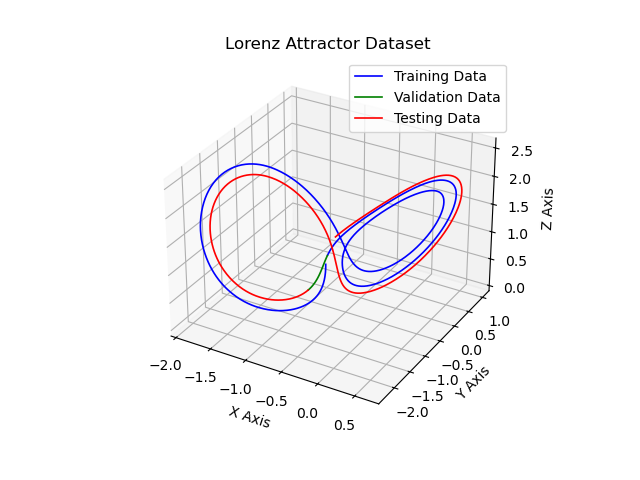
\includegraphics[width=0.75\textwidth]
        {./Images/Dataset_2/partial_data.png}
        \caption{Lorenz attractor - Range [8600, 10500] }
        \label{fig:dataset_2_partial_data}
    \end{figure}
    %
    \begin{figure}[ht!]
        \centering
        \begin{minipage}{0.31\textwidth}
            \centering
            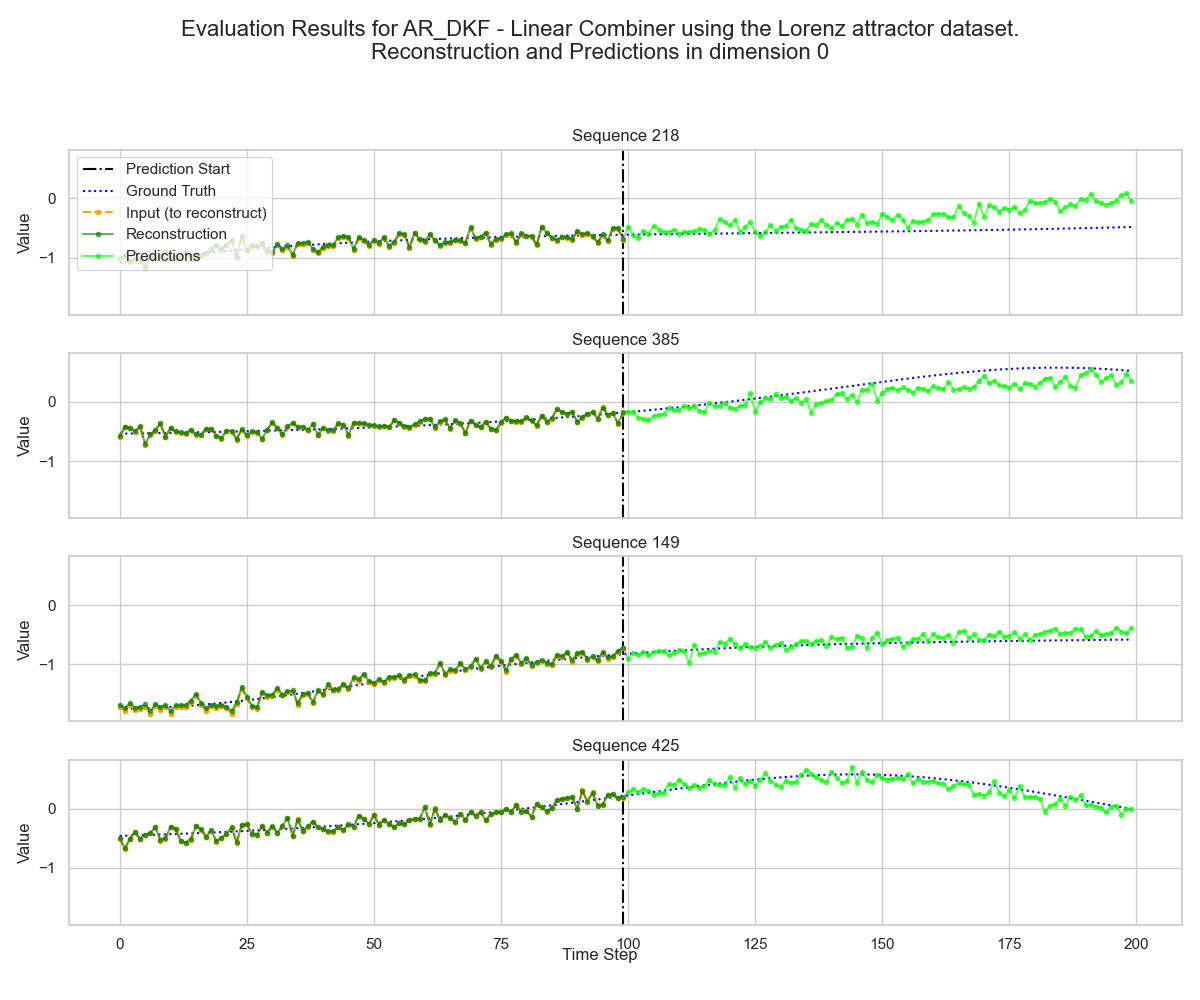
\includegraphics[width=1\textwidth]{./Images/Dataset_2/AR_DKF_1_dim_0.png}
            \subcaption{Reconstruction and Prediction in the 1st dimension.}
            \label{fig:dataset_2_AR_DKF_1_dim_0}
        \end{minipage}
        \hfill
        \begin{minipage}{0.31\textwidth}
            \centering
            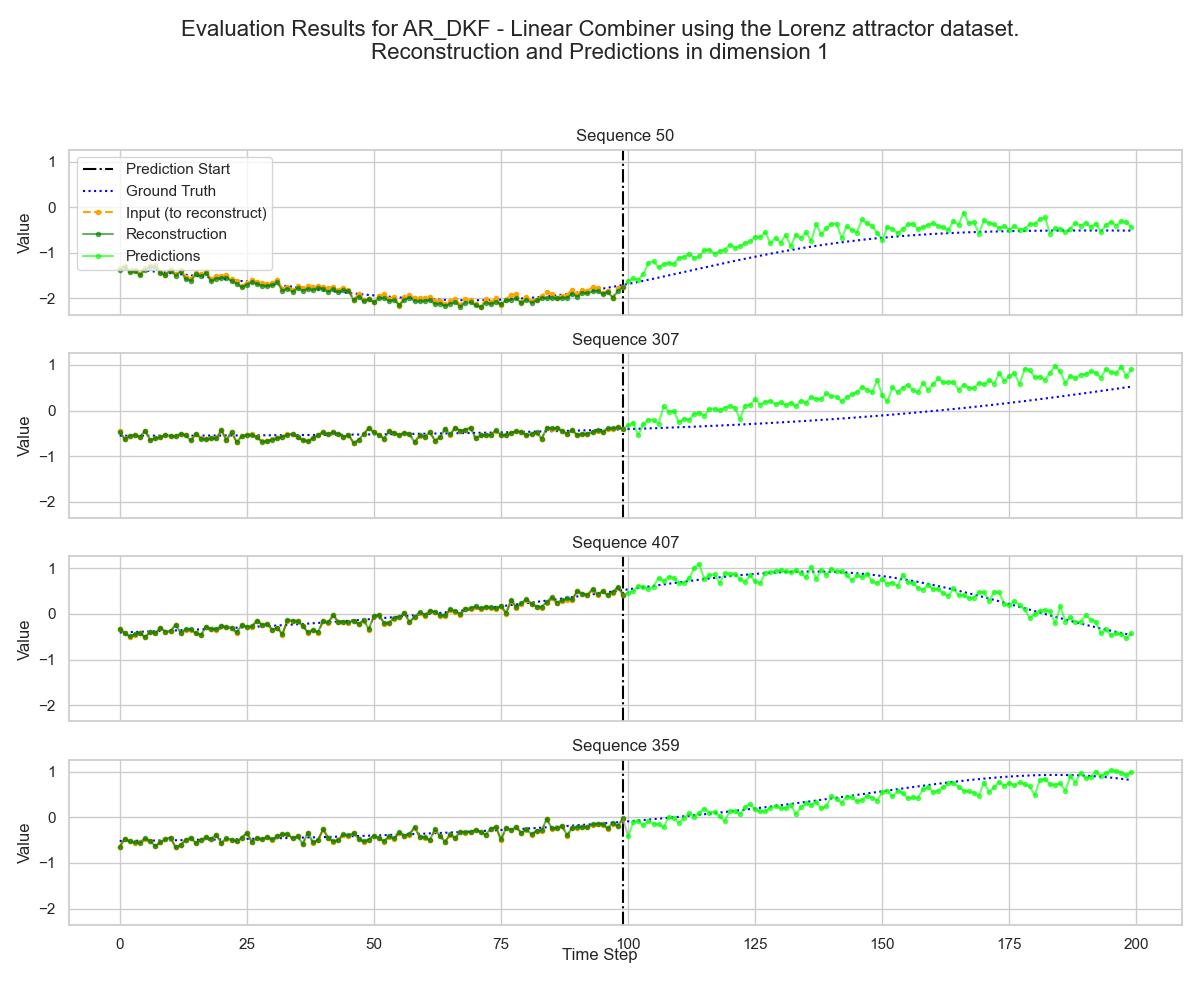
\includegraphics[width=1\textwidth]{./Images/Dataset_2/AR_DKF_1_dim_1.png}
            \subcaption{Reconstruction and Prediction in the 2nd dimension.}
            \label{fig:dataset_2_AR_DKF_1_dim_1}
        \end{minipage}
        \hfill
        \begin{minipage}{0.31\textwidth}
            \centering
            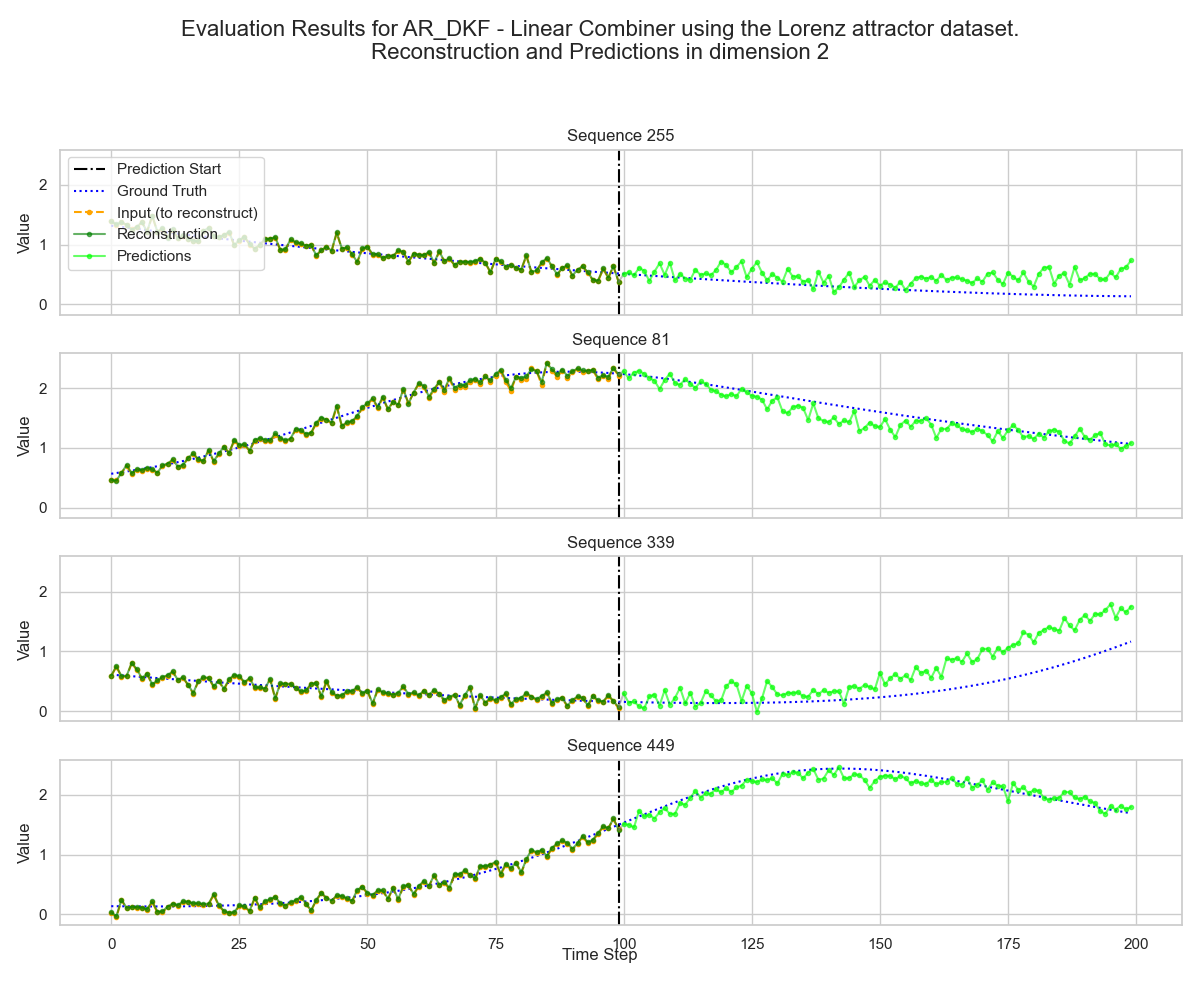
\includegraphics[width=1\textwidth]{./Images/Dataset_2/AR_DKF_1_dim_2.png}
            \subcaption{Reconstruction and Prediction in the 3rd dimension.}
            \label{fig:dataset_2_AR_DKF_1_dim_2}
        \end{minipage}
        \caption{Examples of Reconstruction and Prediction for the
        AR DKF model.}
        \label{fig:dataset_2_AR_DKF_1_all_dims}
    \end{figure}
    
    \begin{figure}[ht!]
        \centering
        \begin{minipage}{0.31\textwidth}
            \centering
            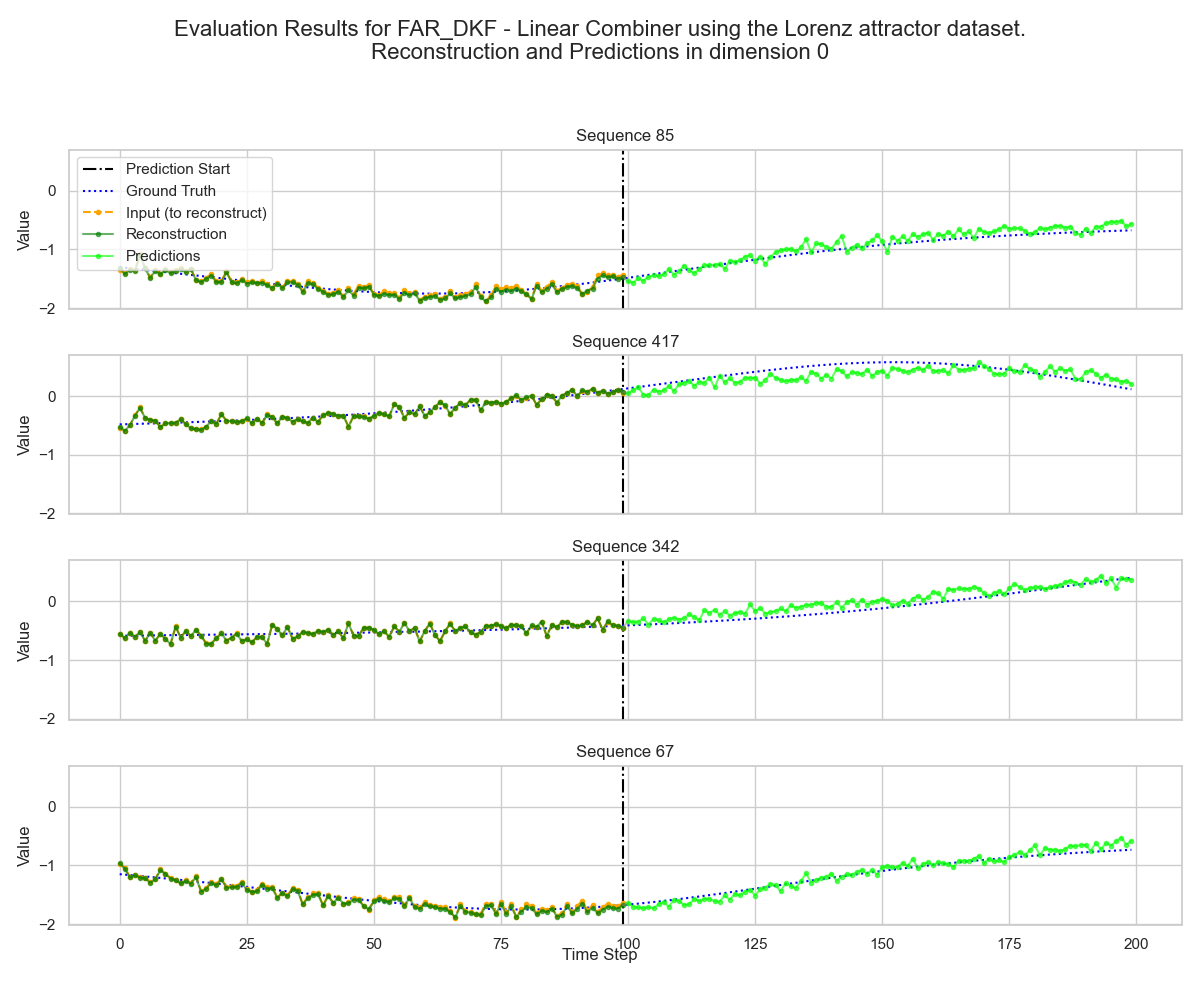
\includegraphics[width=1\textwidth]{./Images/Dataset_2/FAR_DKF_1_dim_0.png}
            \subcaption{Reconstruction and Prediction in the 1st dimension.}
            \label{fig:dataset_2_FAR_DKF_1_dim_0}
        \end{minipage}
        \hfill
        \begin{minipage}{0.31\textwidth}
            \centering
            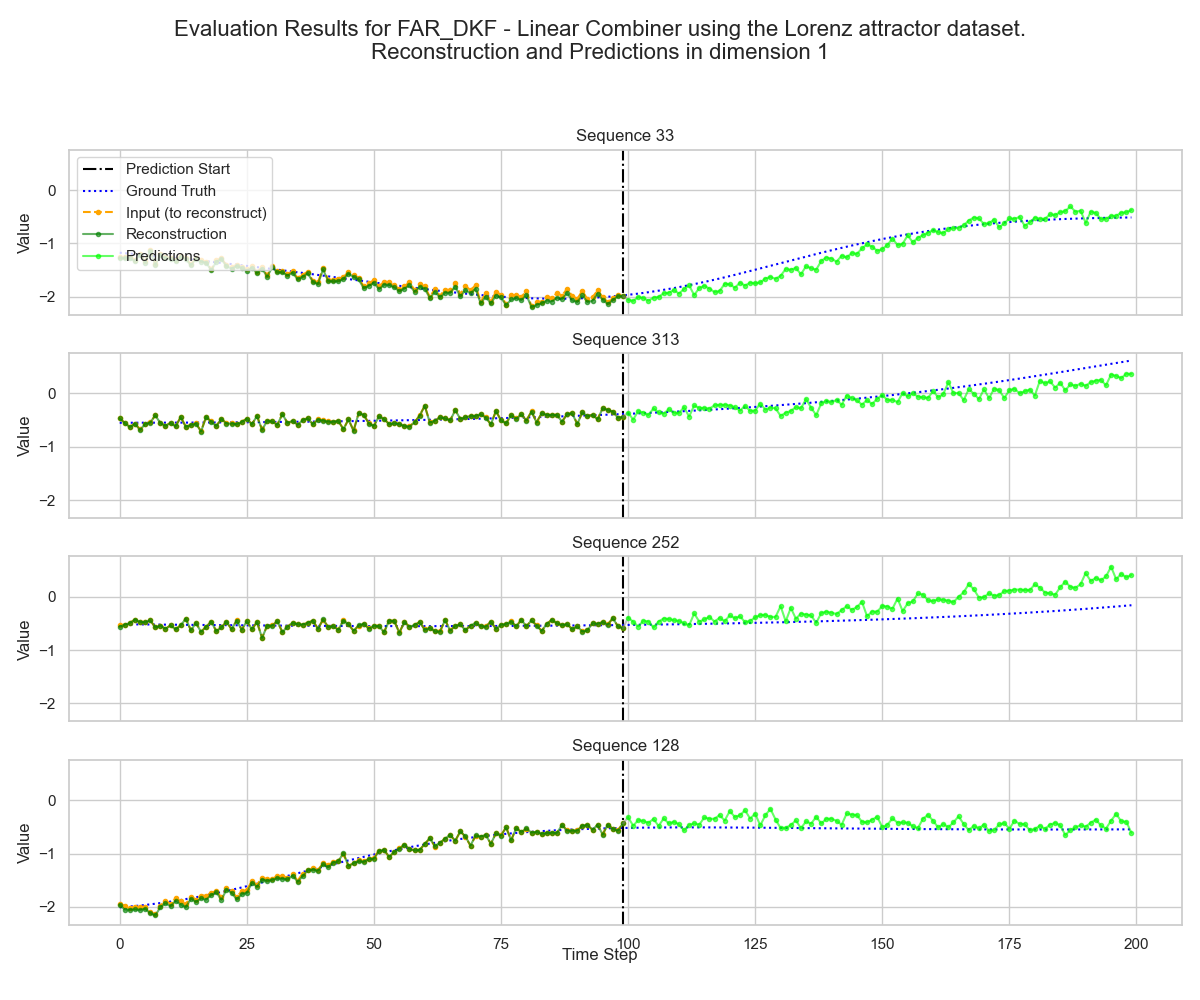
\includegraphics[width=1\textwidth]{./Images/Dataset_2/FAR_DKF_1_dim_1.png}
            \subcaption{Reconstruction and Prediction in the 2nd dimension.}
            \label{fig:dataset_2_FAR_DKF_1_dim_1}
        \end{minipage}
        \hfill
        \begin{minipage}{0.31\textwidth}
            \centering
            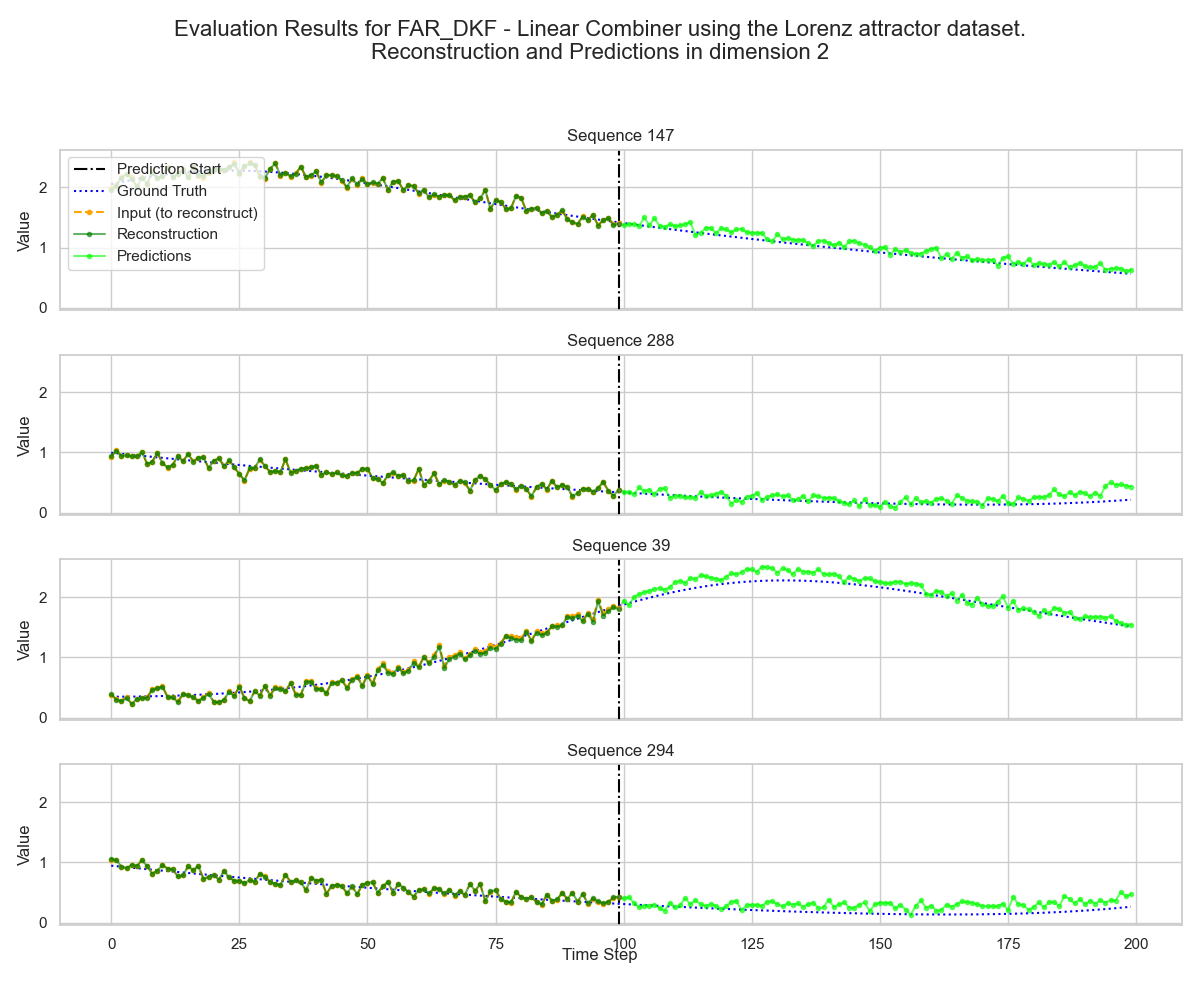
\includegraphics[width=1\textwidth]{./Images/Dataset_2/FAR_DKF_1_dim_2.png}
            \subcaption{Reconstruction and Prediction in the 3rd dimension.}
            \label{fig:dataset_2_FAR_DKF_1_dim_2}
        \end{minipage}
        \caption{Examples of Reconstruction and Prediction for the
        FAR DKF model.}
        \label{fig:dataset_2_FAR_DKF_1_all_dims}
    \end{figure}
    
    \begin{figure}[ht!]
        \centering
        \begin{minipage}{0.31\textwidth}
            \centering
            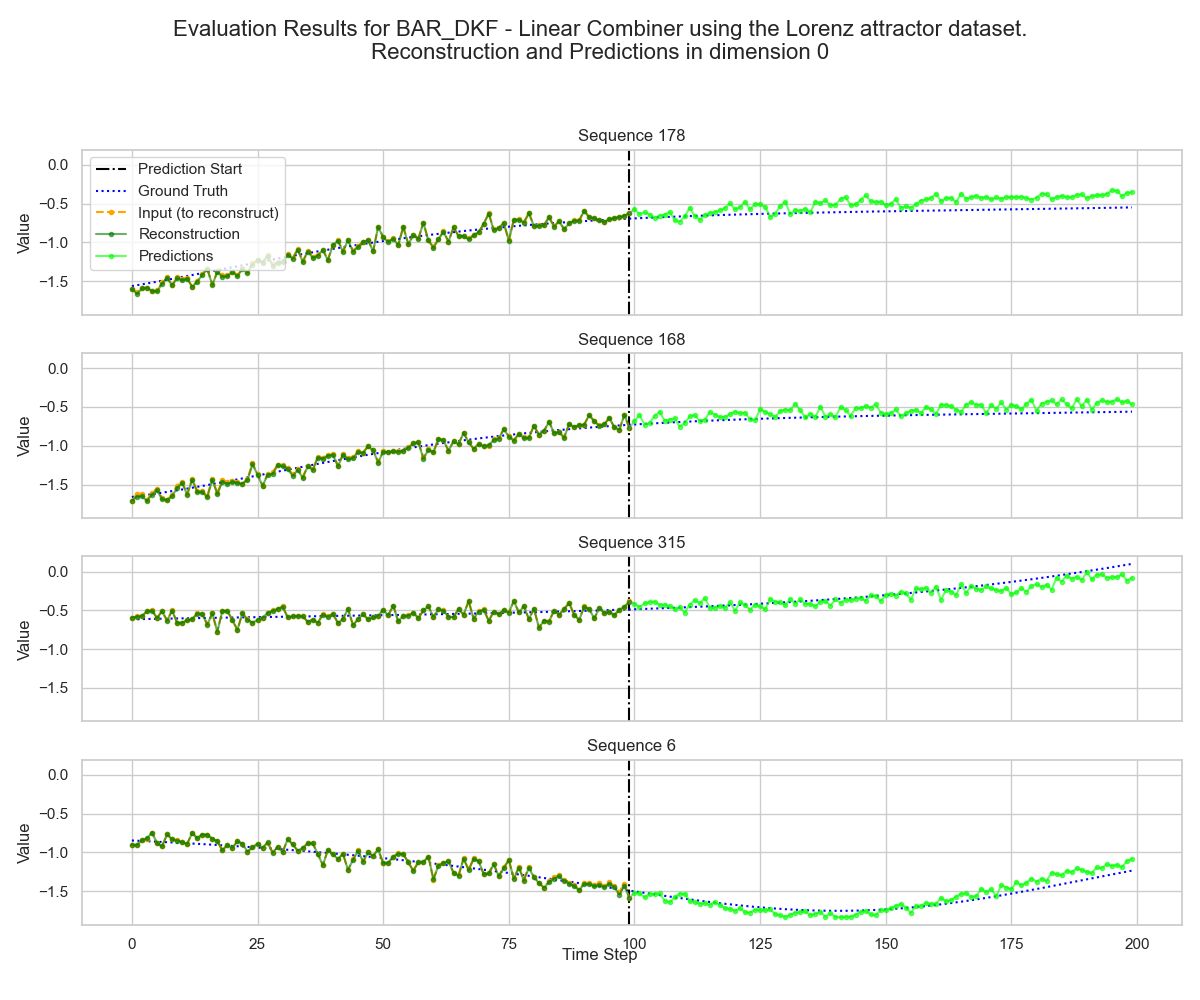
\includegraphics[width=1\textwidth]{./Images/Dataset_2/BAR_DKF_1_dim_0.png}
            \subcaption{Reconstruction and Prediction in the 1st dimension.}
            \label{fig:dataset_2_BAR_DKF_1_dim_0}
        \end{minipage}
        \hfill
        \begin{minipage}{0.31\textwidth}
            \centering
            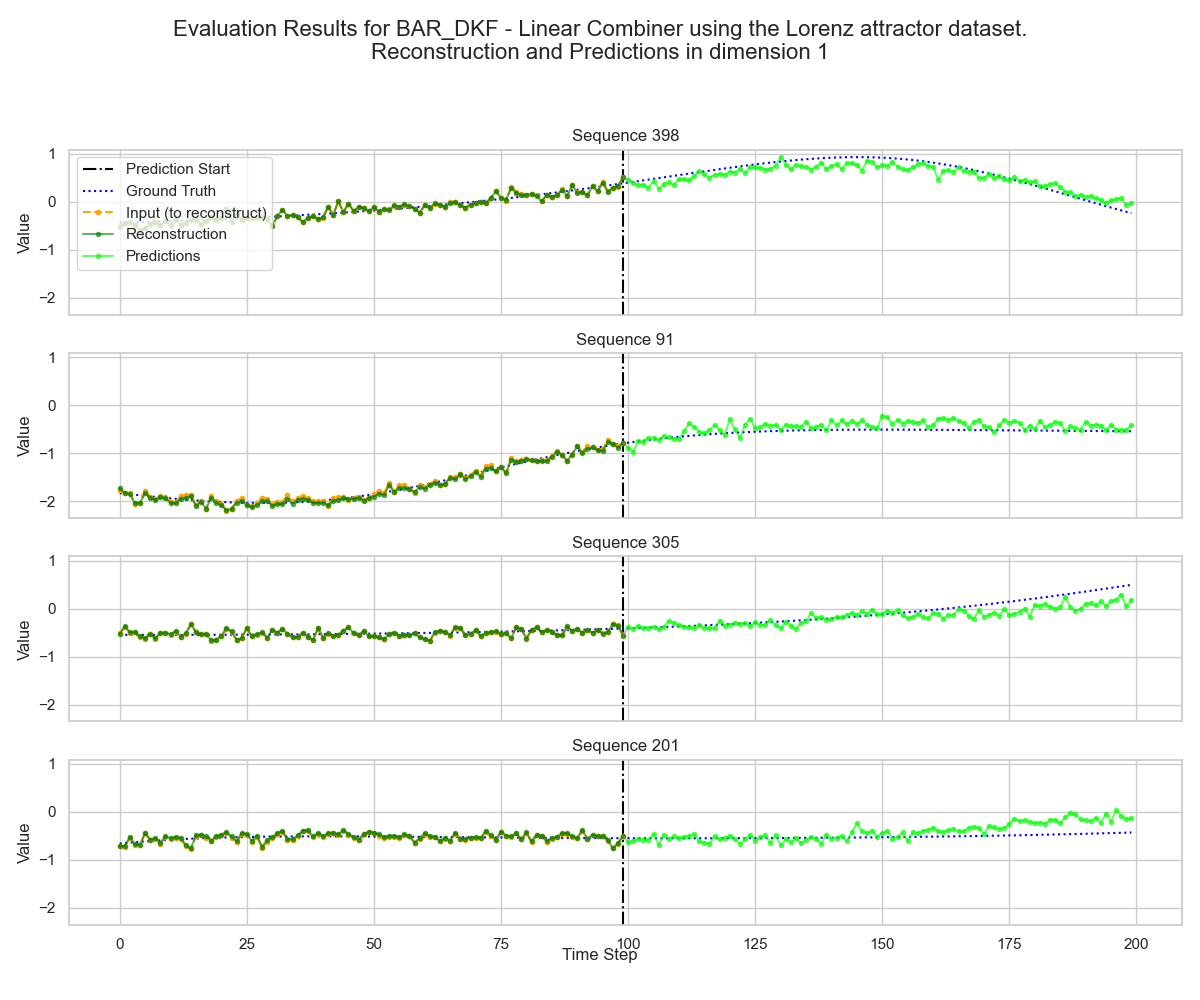
\includegraphics[width=1\textwidth]{./Images/Dataset_2/BAR_DKF_1_dim_1.png}
            \subcaption{Reconstruction and Prediction in the 2nd dimension.}
            \label{fig:dataset_2_BAR_DKF_1_dim_1}
        \end{minipage}
        \hfill
        \begin{minipage}{0.31\textwidth}
            \centering
            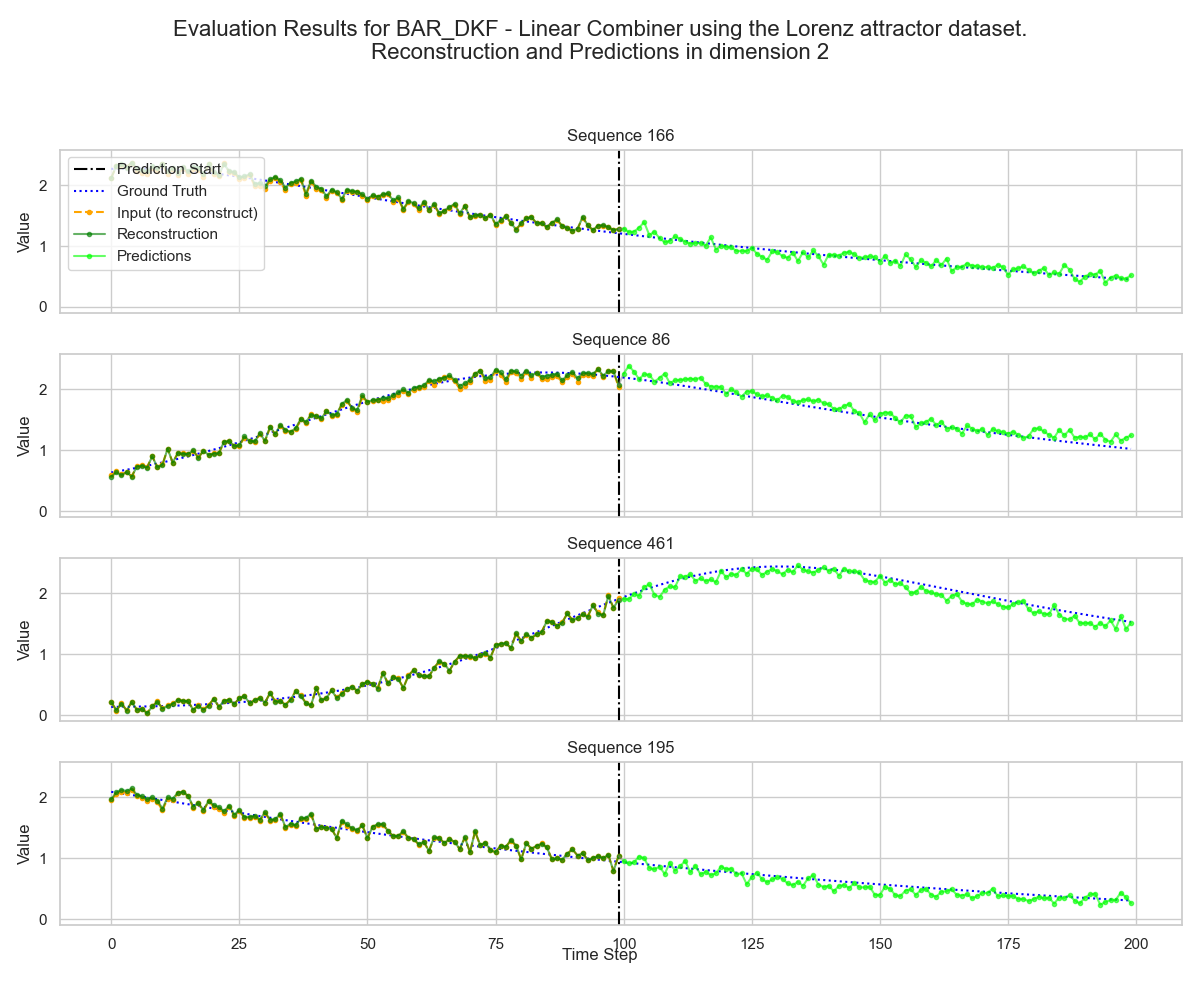
\includegraphics[width=1\textwidth]{./Images/Dataset_2/BAR_DKF_1_dim_2.png}
            \subcaption{Reconstruction and Prediction in the 3rd dimension.}
            \label{fig:dataset_2_BAR_DKF_1_dim_2}
        \end{minipage}
        \caption{Examples of Reconstruction and Prediction for the
        BAR DKF model.}
        \label{fig:dataset_2_BAR_DKF_1_all_dims}
    \end{figure}
    
    \begin{figure}[ht!]
        \centering
        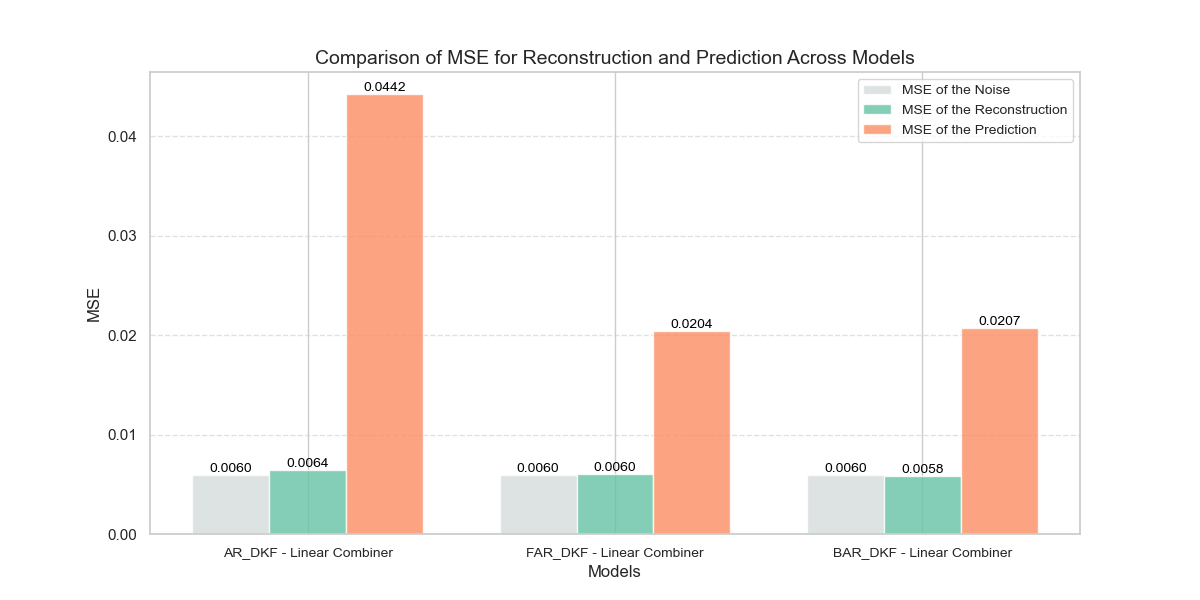
\includegraphics[width=0.75\textwidth]
        {./Images/Dataset_2/mse_comparison.png}
        \caption{Reconstruction and Prediction MSE Comparison for
        AR DKF, FAR DKF, and BAR DKF
        on dataset 2.}
        \label{fig:dataset_2_mse_comparison}
    \end{figure}
    
    \begin{figure}[ht!]
        \centering
        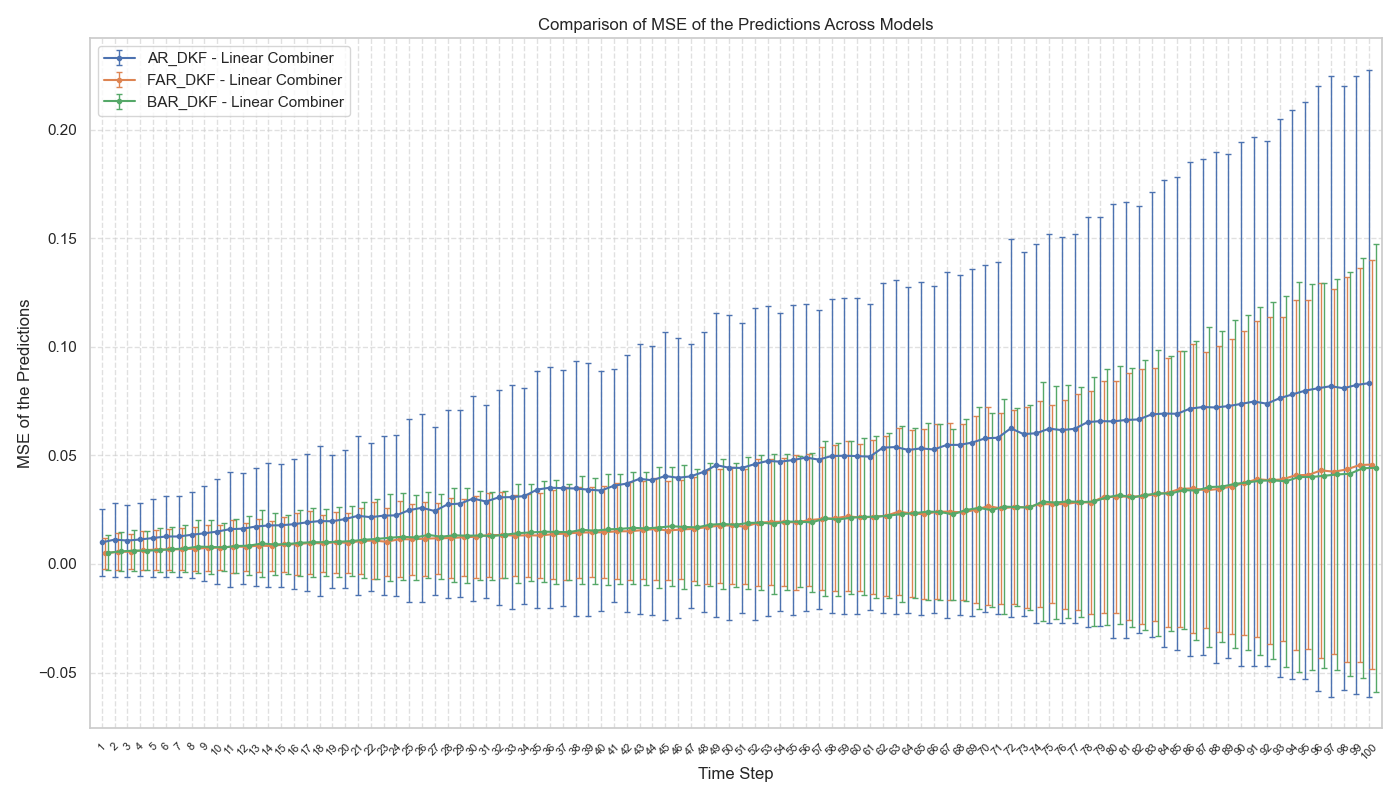
\includegraphics[width=1\textwidth]
        {./Images/Dataset_2/mse_pred_comparison.png}
        \caption{MSE Comparison for AR DKF, FAR DKF, and
        BAR DKF for each prediction points of test sequences of
        dataset 2.}
        \label{fig:dataset_2_mse_pred_comparison}
    \end{figure}
    %- - - - - - - - - - - - - - - - - - - - - - - - - - - - 
    \FloatBarrier
    \subsubsection*{Dataset 3}
    
    The dataset (\textit{before the addition of Gaussian noise}) is shown
    in figure \ref{fig:dataset_3_partial_data} below.\\
    
    \begin{figure}[ht!]
        \centering
        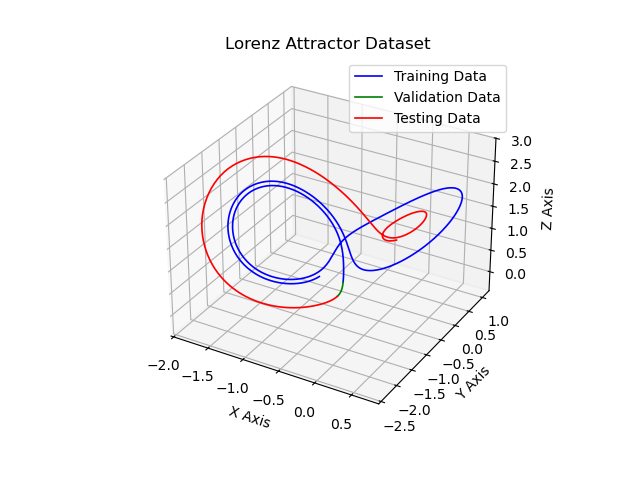
\includegraphics[width=0.75\textwidth]
        {./Images/Dataset_3/partial_data.png}
        \caption{Lorenz attractor - Range [11000, 13000] }
        \label{fig:dataset_3_partial_data}
    \end{figure}
    
    \begin{figure}[ht!]
        \centering
        \begin{minipage}{0.31\textwidth}
            \centering
            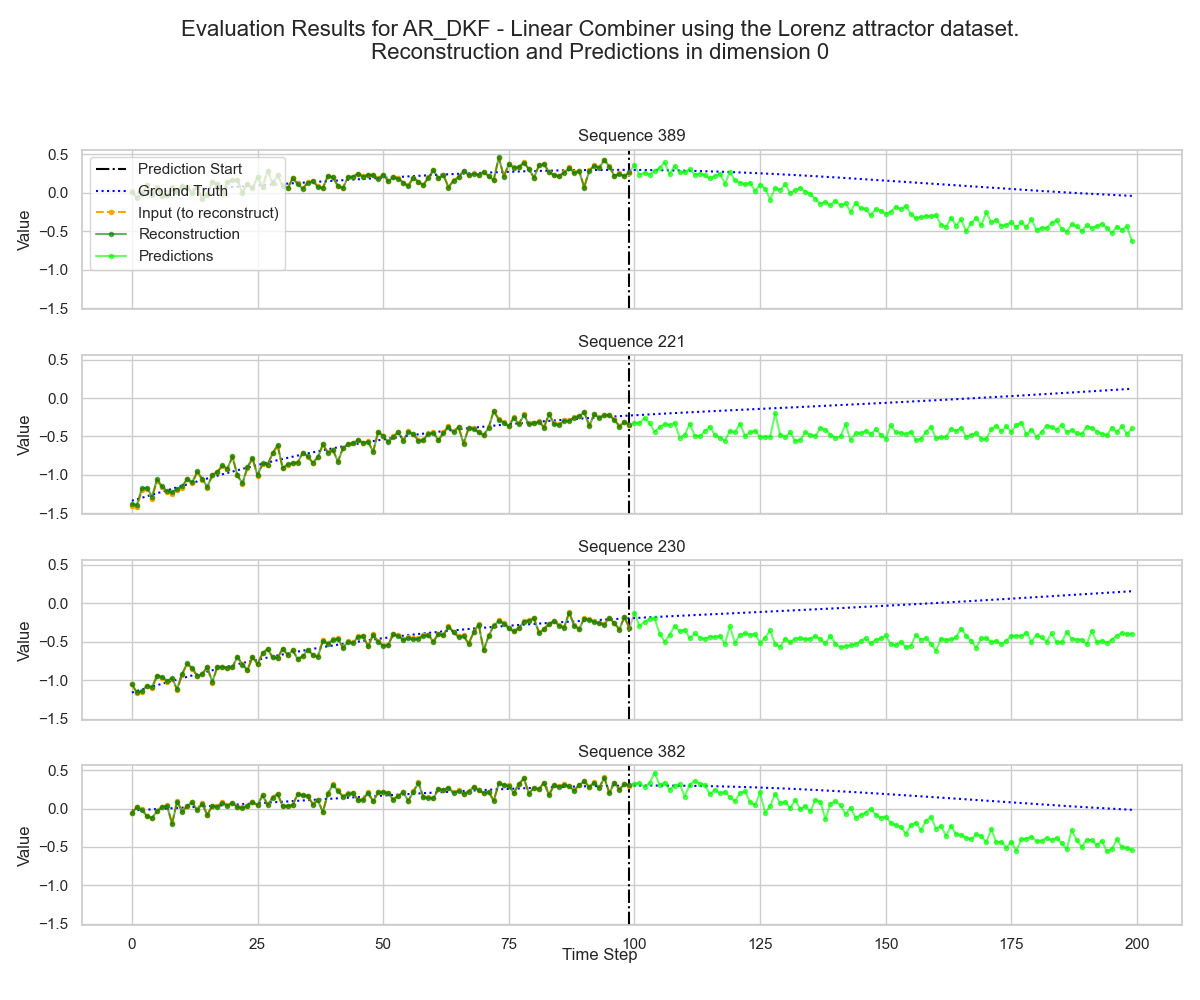
\includegraphics[width=1\textwidth]{./Images/Dataset_3/AR_DKF_1_dim_0.png}
            \subcaption{Reconstruction and Prediction in the 1st dimension.}
            \label{fig:dataset_3_AR_DKF_1_dim_0}
        \end{minipage}
        \hfill
        \begin{minipage}{0.31\textwidth}
            \centering
            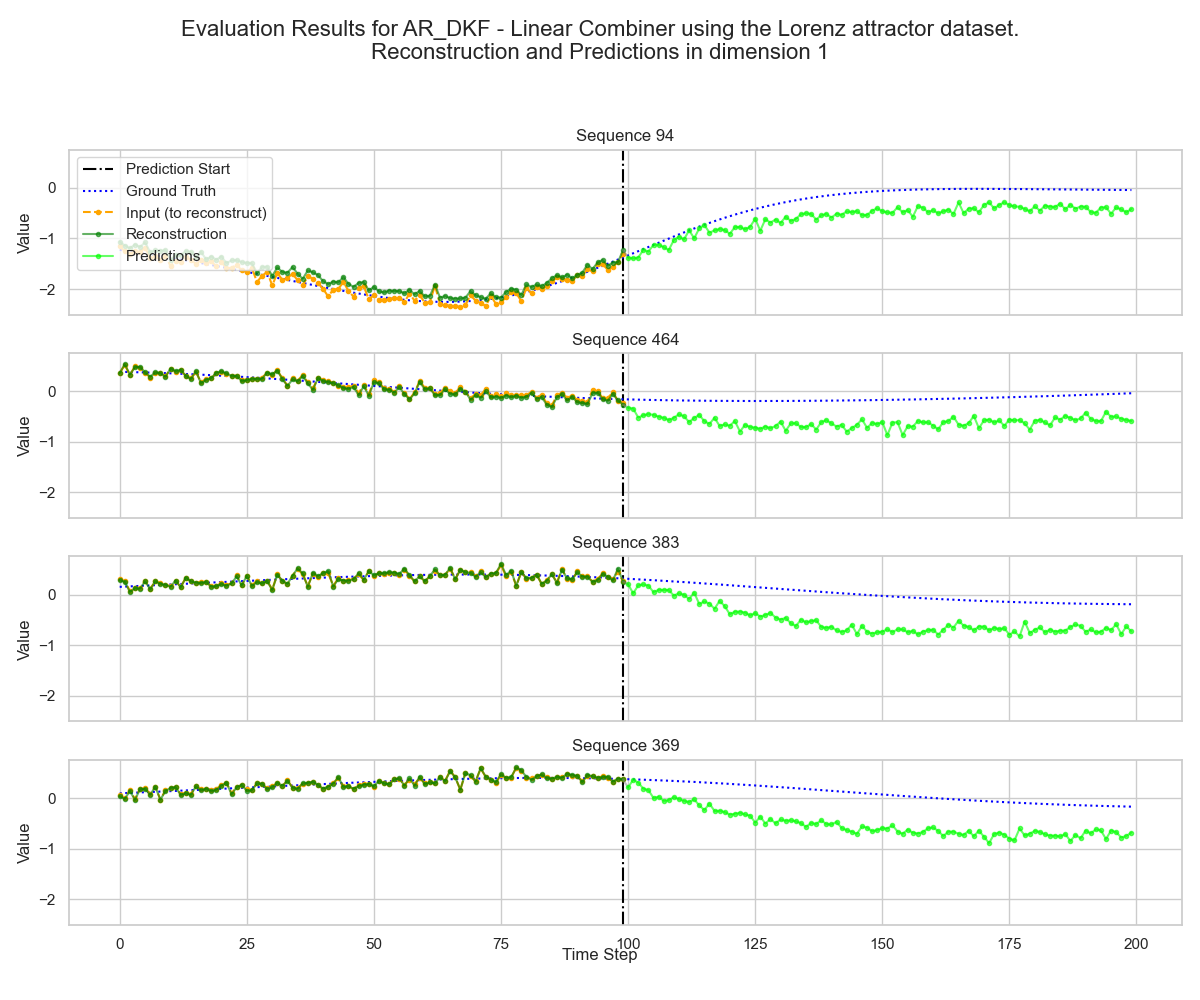
\includegraphics[width=1\textwidth]{./Images/Dataset_3/AR_DKF_1_dim_1.png}
            \subcaption{Reconstruction and Prediction in the 2nd dimension.}
            \label{fig:dataset_3_AR_DKF_1_dim_1}
        \end{minipage}
        \hfill
        \begin{minipage}{0.31\textwidth}
            \centering
            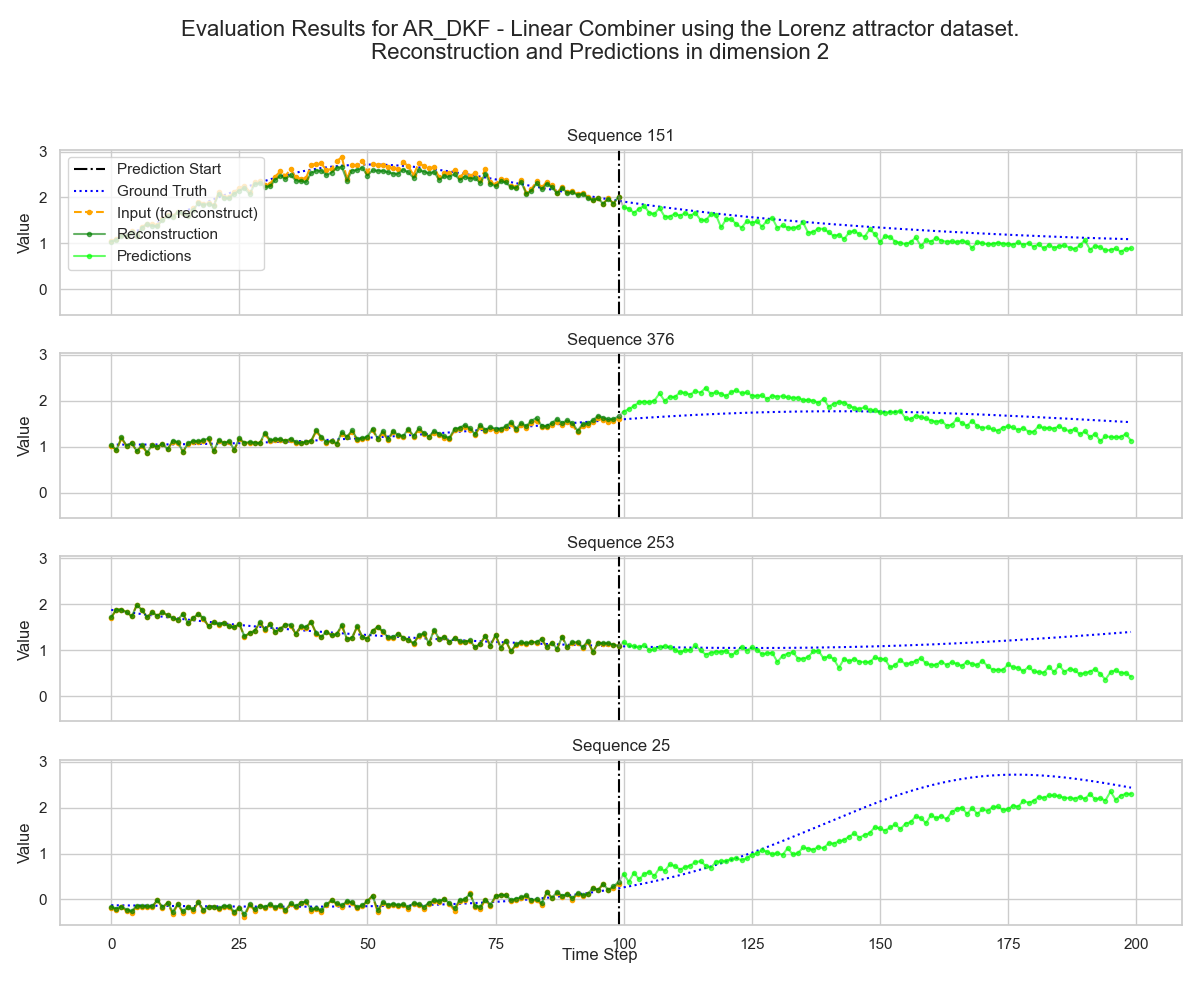
\includegraphics[width=1\textwidth]{./Images/Dataset_3/AR_DKF_1_dim_2.png}
            \subcaption{Reconstruction and Prediction in the 3rd dimension.}
            \label{fig:dataset_3_AR_DKF_1_dim_2}
        \end{minipage}
        \caption{Examples of Reconstruction and Prediction for the
        AR DKF model.}
        \label{fig:dataset_3_AR_DKF_1_all_dims}
    \end{figure}
    
    \begin{figure}[ht!]
        \centering
        \begin{minipage}{0.31\textwidth}
            \centering
            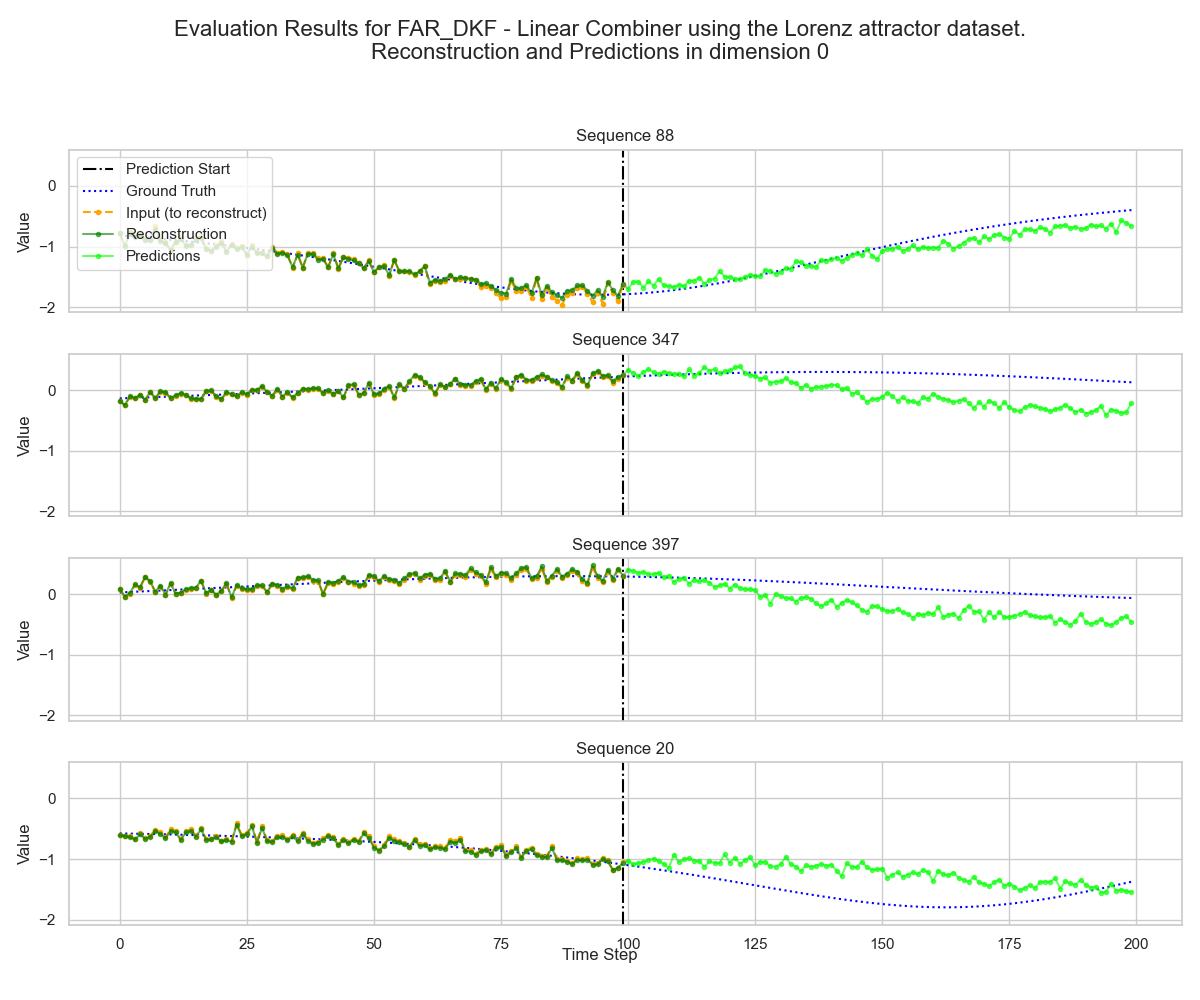
\includegraphics[width=1\textwidth]{./Images/Dataset_3/FAR_DKF_1_dim_0.png}
            \subcaption{Reconstruction and Prediction in the 1st dimension.}
            \label{fig:dataset_3_FAR_DKF_1_dim_0}
        \end{minipage}
        \hfill
        \begin{minipage}{0.31\textwidth}
            \centering
            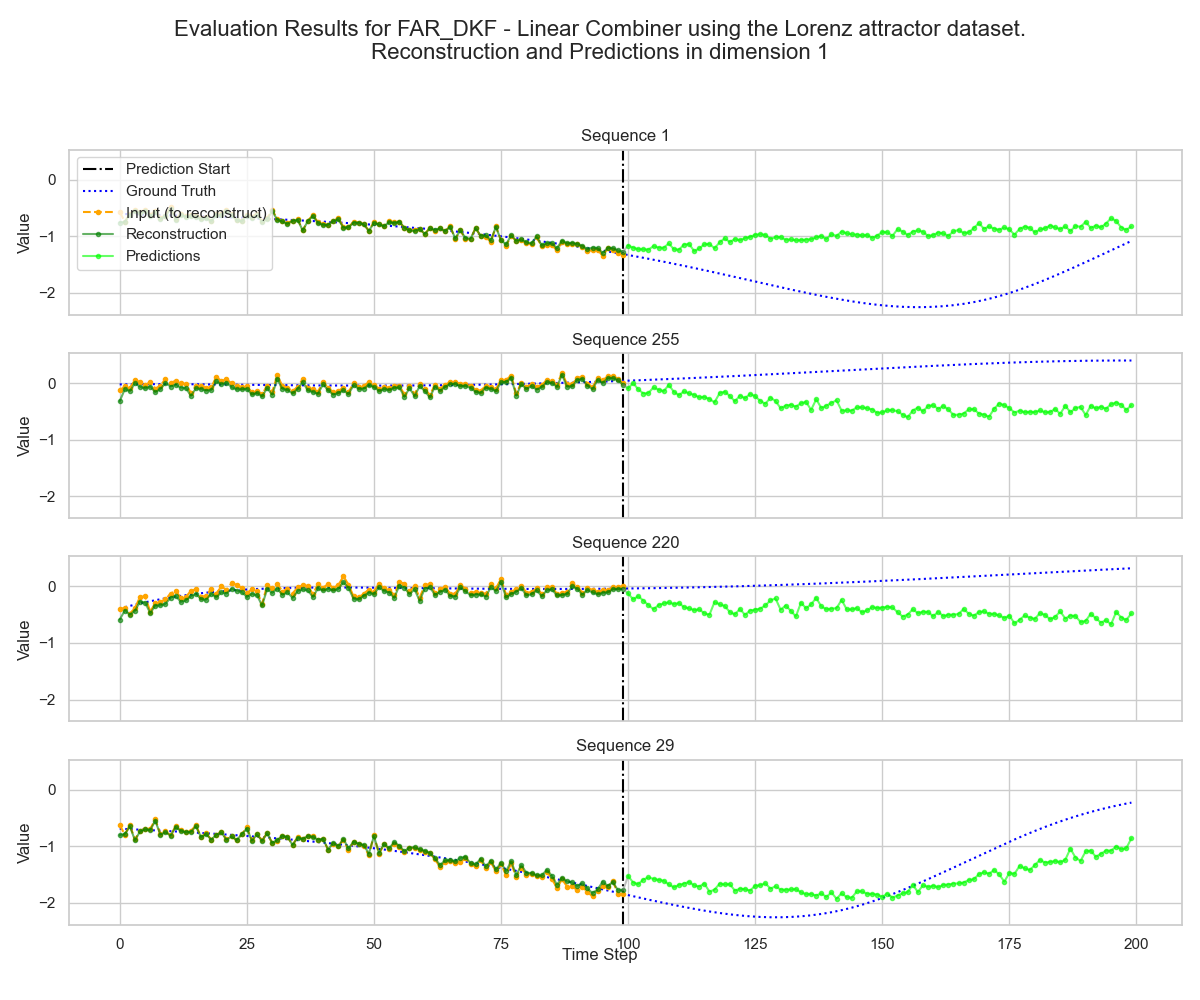
\includegraphics[width=1\textwidth]{./Images/Dataset_3/FAR_DKF_1_dim_1.png}
            \subcaption{Reconstruction and Prediction in the 2nd dimension.}
            \label{fig:dataset_3_FAR_DKF_1_dim_1}
        \end{minipage}
        \hfill
        \begin{minipage}{0.31\textwidth}
            \centering
            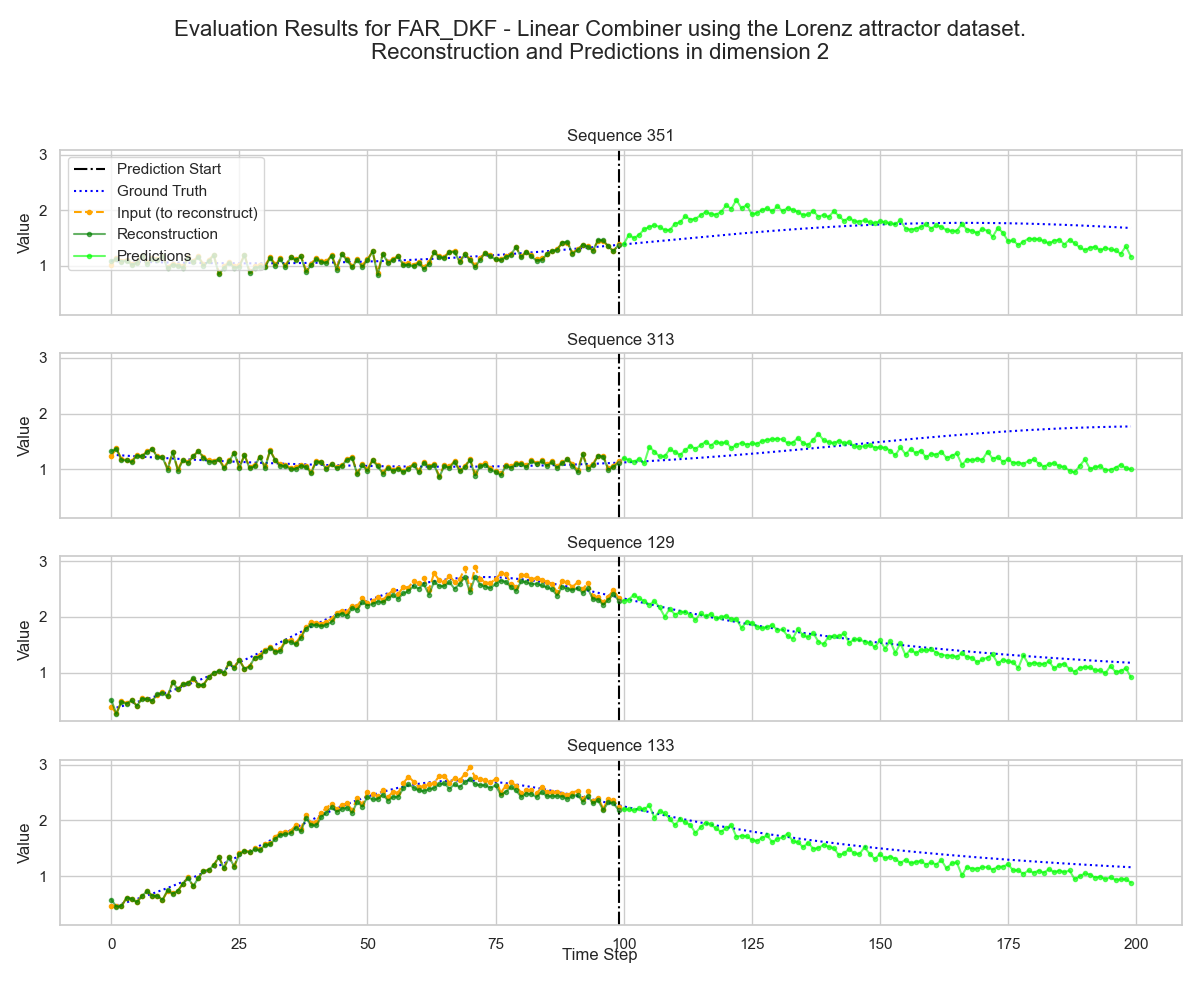
\includegraphics[width=1\textwidth]{./Images/Dataset_3/FAR_DKF_1_dim_2.png}
            \subcaption{Reconstruction and Prediction in the 3rd dimension.}
            \label{fig:dataset_3_FAR_DKF_1_dim_2}
        \end{minipage}
        \caption{Examples of Reconstruction and Prediction for the
        FAR DKF model.}
        \label{fig:dataset_3_FAR_DKF_1_all_dims}
    \end{figure}
    
    \begin{figure}[ht!]
        \centering
        \begin{minipage}{0.31\textwidth}
            \centering
            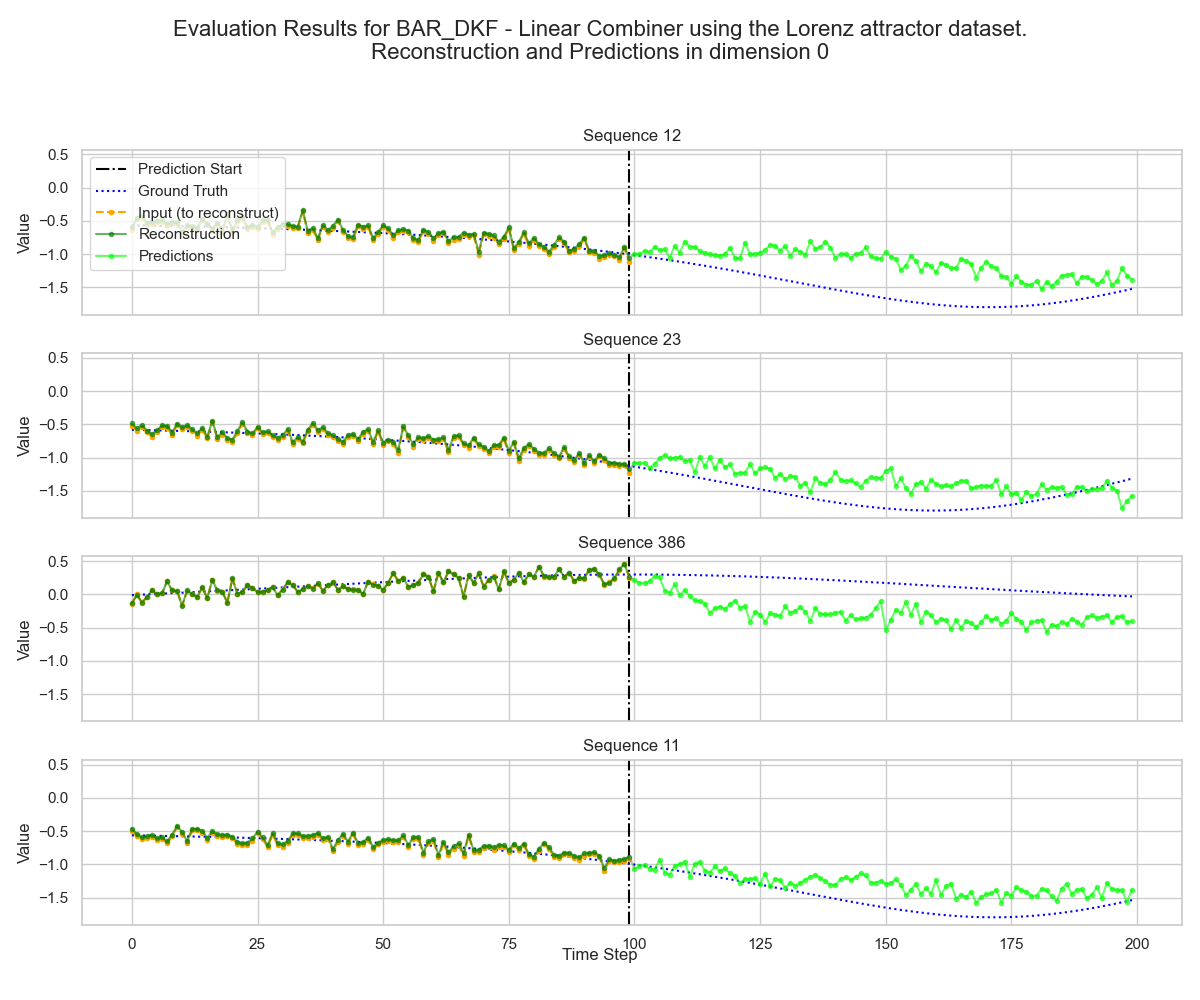
\includegraphics[width=1\textwidth]{./Images/Dataset_3/BAR_DKF_1_dim_0.png}
            \subcaption{Reconstruction and Prediction in the 1st dimension.}
            \label{fig:dataset_3_BAR_DKF_1_dim_0}
        \end{minipage}
        \hfill
        \begin{minipage}{0.31\textwidth}
            \centering
            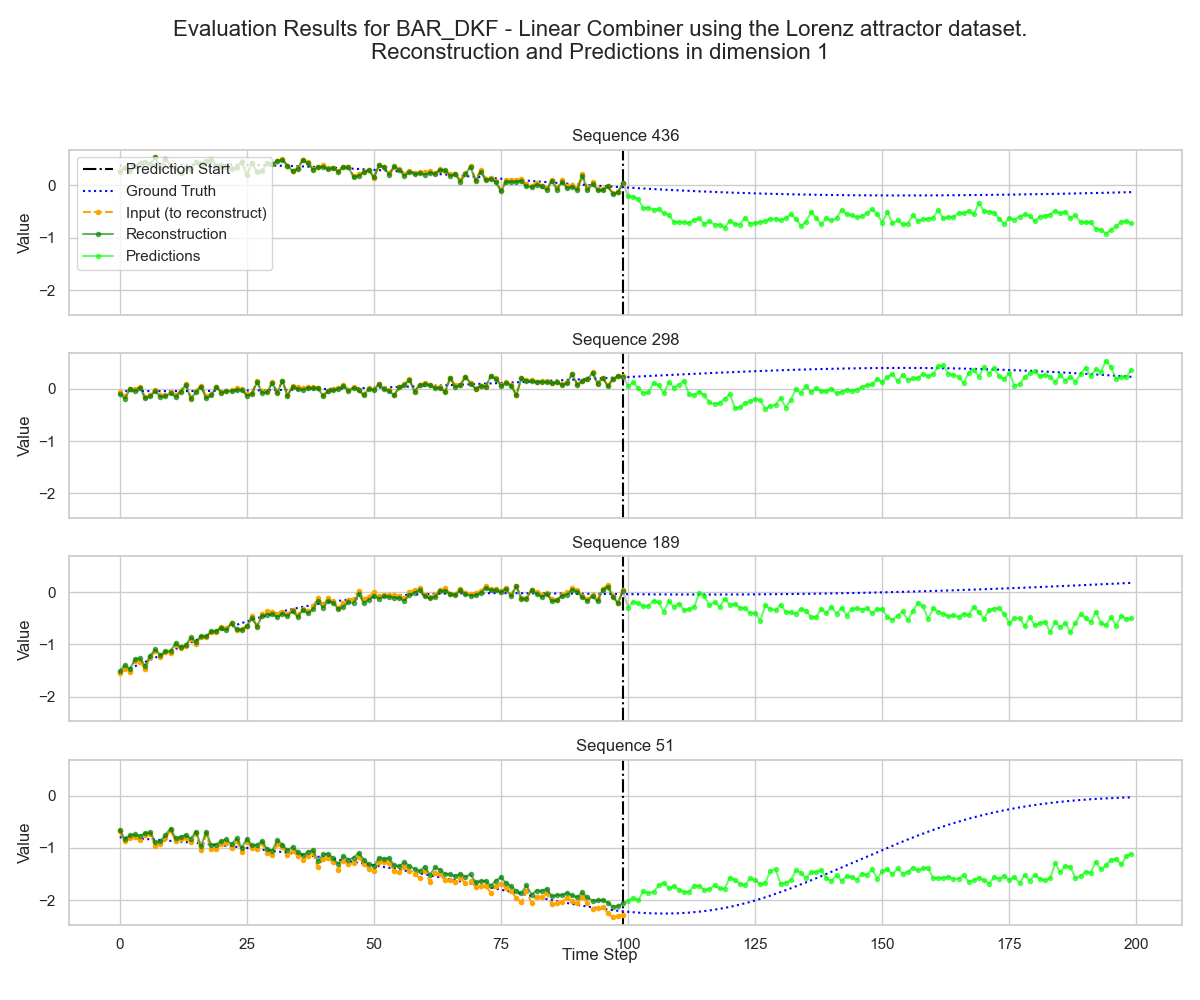
\includegraphics[width=1\textwidth]{./Images/Dataset_3/BAR_DKF_1_dim_1.png}
            \subcaption{Reconstruction and Prediction in the 2nd dimension.}
            \label{fig:dataset_3_BAR_DKF_1_dim_1}
        \end{minipage}
        \hfill
        \begin{minipage}{0.31\textwidth}
            \centering
            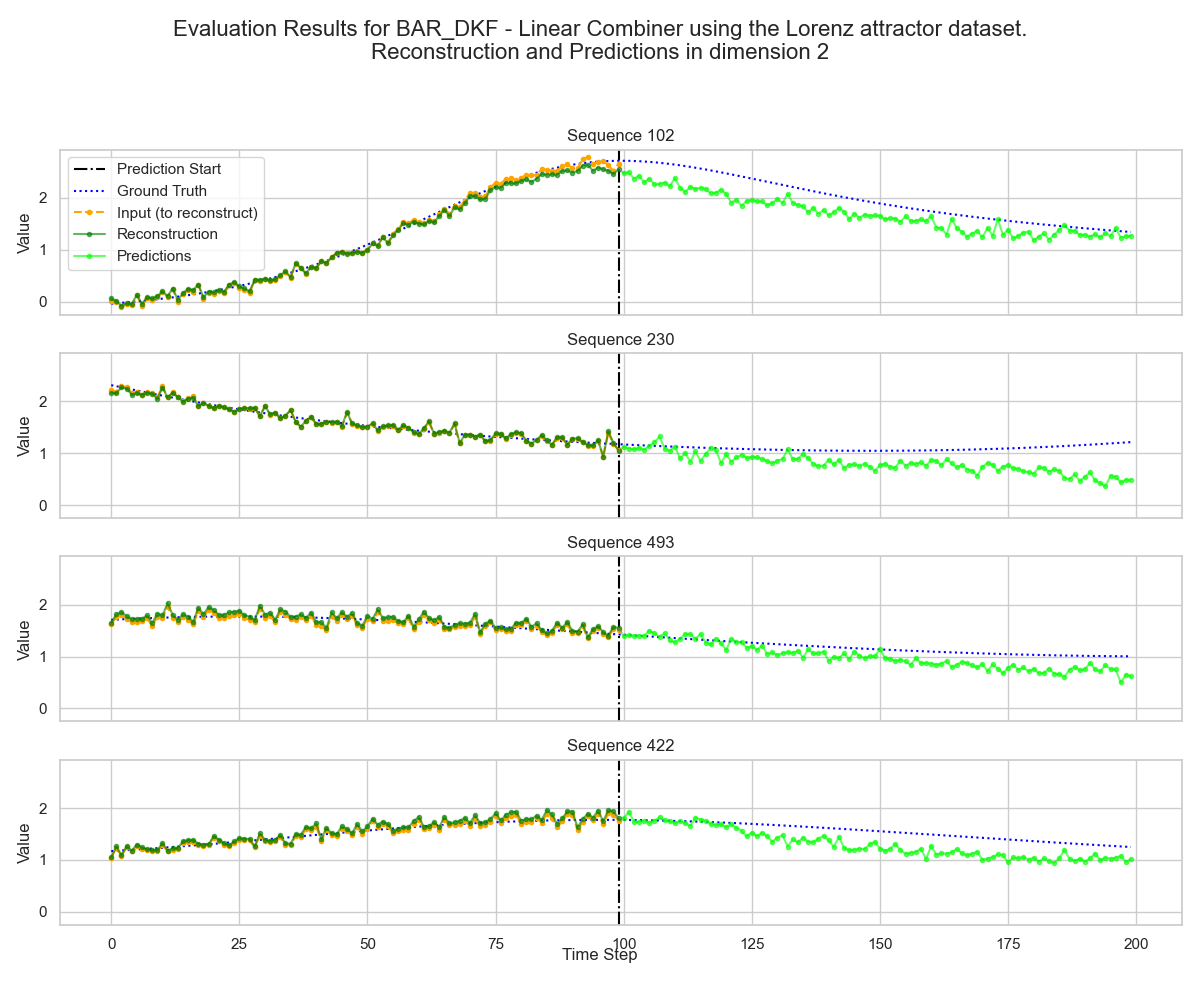
\includegraphics[width=1\textwidth]{./Images/Dataset_3/BAR_DKF_1_dim_2.png}
            \subcaption{Reconstruction and Prediction in the 3rd dimension.}
            \label{fig:dataset_3_BAR_DKF_1_dim_2}
        \end{minipage}
        \caption{Examples of Reconstruction and Prediction for the
        BAR DKF model.}
        \label{fig:dataset_3_BAR_DKF_1_all_dims}
    \end{figure}
    
    \begin{figure}[ht!]
        \centering
        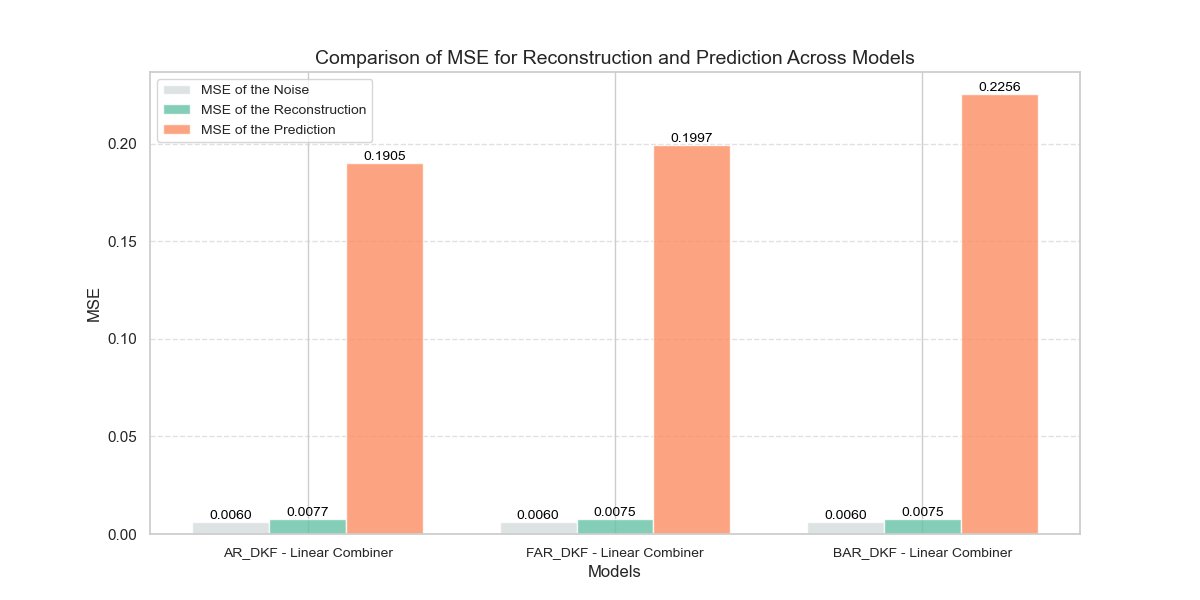
\includegraphics[width=0.75\textwidth]
        {./Images/Dataset_3/mse_comparison.png}
        \caption{Reconstruction and Prediction MSE Comparison for
        AR DKF, FAR DKF, and BAR DKF
        on dataset 3.}
        \label{fig:dataset_3_mse_comparison}
    \end{figure}
    
    \begin{figure}[ht!]
        \centering
        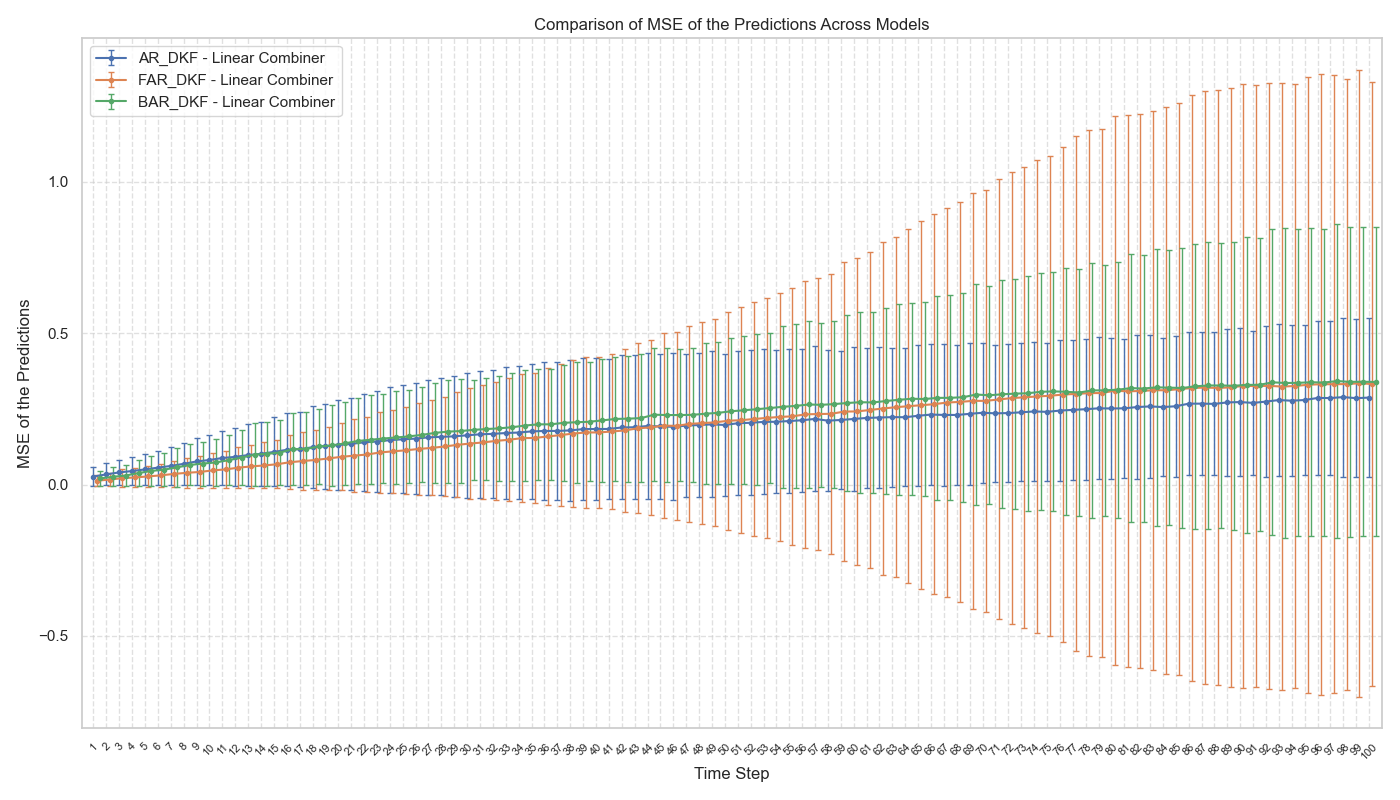
\includegraphics[width=1\textwidth]
        {./Images/Dataset_3/mse_pred_comparison.png}
        \caption{MSE Comparison for AR DKF, FAR DKF, and
        BAR DKF for each prediction points of test sequences of
        dataset 3.}
        \label{fig:dataset_3_mse_pred_comparison}
    \end{figure}

%- - - - - - - - - - - - - - - - - - - - - - - - - - - - - - - - - - - - -
\FloatBarrier
\subsubsection*{Summary of the Lorenz experiments}

The code does not fix a random seed, so each training run starts from
a different initialisation and sees the minibatches in a different
order. Table~\ref{tab:lorenz_mse} gives the forecasting and
reconstruction errors over the four runs of each experiment.

\begin{table}[ht!]
\centering
\small
\begin{tabular}{|c|c|c|c|}
\hline
Dataset & Model & Prediction MSE: mean (std.\ dev.) &
Runs with the lowest error \\ \hline
1 & AR DKF  & 0.0357 (0.0202) & 2 of 4 \\
  & FAR DKF & 0.0315 (0.0063) & 1 of 4 \\
  & BAR DKF & 0.0280 (0.0044) & 1 of 4 \\ \hline
2 & AR DKF  & 0.0244 (0.0135) & 3 of 4 \\
  & FAR DKF & 0.0361 (0.0232) & 1 of 4 \\
  & BAR DKF & 0.0621 (0.0695) & 0 of 4 \\ \hline
3 & AR DKF  & 0.1974 (0.0283) & 1 of 4 \\
  & FAR DKF & 0.1418 (0.0513) & 2 of 4 \\
  & BAR DKF & 0.1711 (0.0597) & 1 of 4 \\ \hline
\end{tabular}
\caption{Lorenz experiments: prediction MSE over four training runs.
The MSE of the noise is 0.0060.}
\label{tab:lorenz_mse}
\end{table}

\begin{itemize}
    \item \textbf{Reconstruction.} In almost every run, all three models
    reconstruct close to the noise level (mean reconstruction MSE between
    0.0050 and 0.0071, except 0.0119 for the AR DKF on dataset 3, due to
    one run at 0.0225). They reproduce the noisy input rather than
    denoise it.
    \item \textbf{Prediction.} The spread between runs of the \emph{same}
    model is as large as the differences between models, and no model is
    consistently best: the AR DKF has the lowest error in three runs out
    of four on dataset 2, the FAR DKF the lowest mean error on dataset 3,
    and on dataset 1 the three means are within one standard deviation of
    each other. The BAR DKF has one poor run on dataset 2 (0.166), which
    drives its mean and spread there. Dataset 3 remains the hardest for
    all models.
\end{itemize}

\subsubsection*{Evaluation of the ELBO on test data}

The theory of Section~\ref{sec:ar_posterior} makes a prediction about
the ELBO, not about forecasting: the FAR DKF and the BAR DKF have
inference networks with the structure of the true posterior
(Proposition~\ref{prop:ar_posterior}); the AR DKF does not. Their gap
$\KL\big(q_\phi \,\|\, p_\theta(\mathbf{z}_{1:T} \mid \mathbf{x}_{1:T})\big)$
between the ELBO and the log-likelihood should therefore be smaller.

To test this, the script \code{evaluate\_elbo.py} evaluates each trained
model on the noisy test sequences (the same noise for all models) with
two quantities, reported per time step:
\begin{itemize}
    \item the ELBO, estimated as during training and averaged over 20
    trajectories per sequence;
    \item the importance-weighted bound \cite{burda2016importance}
    \begin{equation*}
        \mathcal{L}_K = \E\left[\log \frac{1}{K} \sum_{k=1}^{K}
        \frac{p_\theta(\mathbf{x}_{1:T}, \mathbf{z}^{(k)}_{1:T})}
        {q_\phi(\mathbf{z}^{(k)}_{1:T} \mid \mathbf{x}_{1:T})}\right],
        \qquad \mathbf{z}^{(k)}_{1:T} \sim q_\phi(\mathbf{z}_{1:T} \mid
        \mathbf{x}_{1:T}),
    \end{equation*}
    for $K = 1, 10, 100$. It satisfies $\mathcal{L}_1 = \mathcal{L}$
    (the ELBO) and $\mathcal{L}_K \leq \log p_\theta(\mathbf{x}_{1:T})$,
    and it increases with $K$. Hence $\mathcal{L}_{100} - \mathcal{L}$ is
    a \emph{lower bound} on the gap.
\end{itemize}
As a check of the implementation, $\mathcal{L}_1$ agrees with the ELBO
within its confidence interval in every evaluation, and $\mathcal{L}_K$
increases with $K$. The ELBO was evaluated after each of the last three
runs of every dataset (and after the first run for dataset 3).

\begin{table}[ht!]
\centering
\small
\begin{tabular}{|c|c|c|c|}
\hline
Dataset & Model & ELBO: mean (std.\ dev.) &
Gap $\mathcal{L}_{100} - \mathcal{L}$: mean [min, max] \\
\hline
1 & AR DKF  & $-13.8$ (7.5)  & 0.62 [0.58, 0.69] \\
  & FAR DKF & $-23.4$ (8.6)  & 0.65 [0.60, 0.68] \\
  & BAR DKF & $-17.2$ (13.1) & 0.63 [0.56, 0.73] \\ \hline
2 & AR DKF  & $-30.8$ (0.8)  & 0.69 [0.66, 0.70] \\
  & FAR DKF & $-22.9$ (4.7)  & 0.64 [0.62, 0.67] \\
  & BAR DKF & $-25.4$ (12.5) & 0.63 [0.53, 0.69] \\ \hline
3 & AR DKF  & $-41.3$ (8.5)  & 0.80 [0.72, 0.95] \\
  & FAR DKF & $-38.8$ (7.8)  & 0.81 [0.72, 0.95] \\
  & BAR DKF & $-37.5$ (7.4)  & 0.75 [0.73, 0.79] \\ \hline
\end{tabular}
\caption{Lorenz experiments: ELBO and estimated ELBO gap on the test
sequences (in nats per time step; higher ELBO is better). ELBO over
three runs (four for dataset 3); gap over three runs.}
\label{tab:lorenz_elbo}
\end{table}

\begin{itemize}
    \item \textbf{The ELBO varies more between runs than between
    models.} Its standard deviation over runs of the same model is
    mostly between 5 and 13 nats per time step, while the differences between the means
    of the three models are of the same size or smaller, and the model
    with the best ELBO changes from one run to the next. The AR DKF has
    the lowest mean ELBO on dataset 2 (the lowest in two runs out of
    three), yet the lowest forecasting error there: the ELBO and the
    forecasting error measure different things.
    \item \textbf{The estimated gap is the same for the three models}, at
    about 0.6--0.8 nats per time step. With $K = 100$, the
    importance-weighted bound cannot detect the difference that the theory
    predicts. The bound is still rising between $K = 10$ and $K = 100$
    (by 0.2 to 0.4 nats per time step), so it has not converged and the
    true gaps are larger than these estimates. Comparing them would
    require much larger $K$ or a better proposal distribution.
\end{itemize}

\noindent In short, the experiments do not show the advantage of the
FAR DKF and the BAR DKF that the d-separation argument suggests. What
they show clearly is that, at this scale, the variability between
training runs is larger than the differences between the three
inference networks.
